\chapter{\texorpdfstring{Results $\&$ Discussion}{Results \& Discussion}}
\label{Chapter4}
\lhead{Chapter 4. \emph{Results \& Discussion}}
We hereby present the results of the computational investigations of CSH performed throughout this work. The results are organised into the following main sections: \textbf{i}) Structure relaxation and Density of States (DOS) calculations, \textbf{ii}) MLFF generation, \textbf{iii}) Themodynamic properties of CSH, and \textbf{iv}) Transferability of MLFFs and thermal expansion coefficient of CSH. 
 
\section{Structure Relaxation and Density of States (DOS) calculations}
\label{sec:bulk-params-dos}
The initial stage of our computational study on CSH focused on establishing optimal parameters for VASP calculations. In particular, we determined the optimal plane-wave cut-off energy and Brillouin zone sampling (k-point mesh) through convergence tests, ensuring a balance between accuracy and computational cost. Following structural relaxation with these parameters, the DOS was computed to assess the insulating (ceramic) nature of CSH. The results of these convergence analyses and DOS calculations are presented in this section.
\subsection{Cut-off Energy}
The cut-off energy is essential in VASP calculations as it determines the maximum kinetic energy of the plane-wave basis set. As such, it ensures the completeness of this basis set and the accurate description of the electroic structure of the system.  The cut-off energy convergence test herein presented was conducted using the PBEsol functional. As shown in Figure \ref{cutoff-energy}, an optimal $E_{\text{cut}}$ is achieved at 800 eV, where the convergence criteria of 1 meV/atom is satisfied. The notably high cut-off energy can be atributed to the presence of heavy elements in the CSH structure, such as Calcium (Ca) and Silicon (Si), which require a high cut-off energy value\supercite{zotero-item-698}. All the subsequent VASP calculations were performed using this cut-off energy.
\begin{figure}[H]
    \centering
    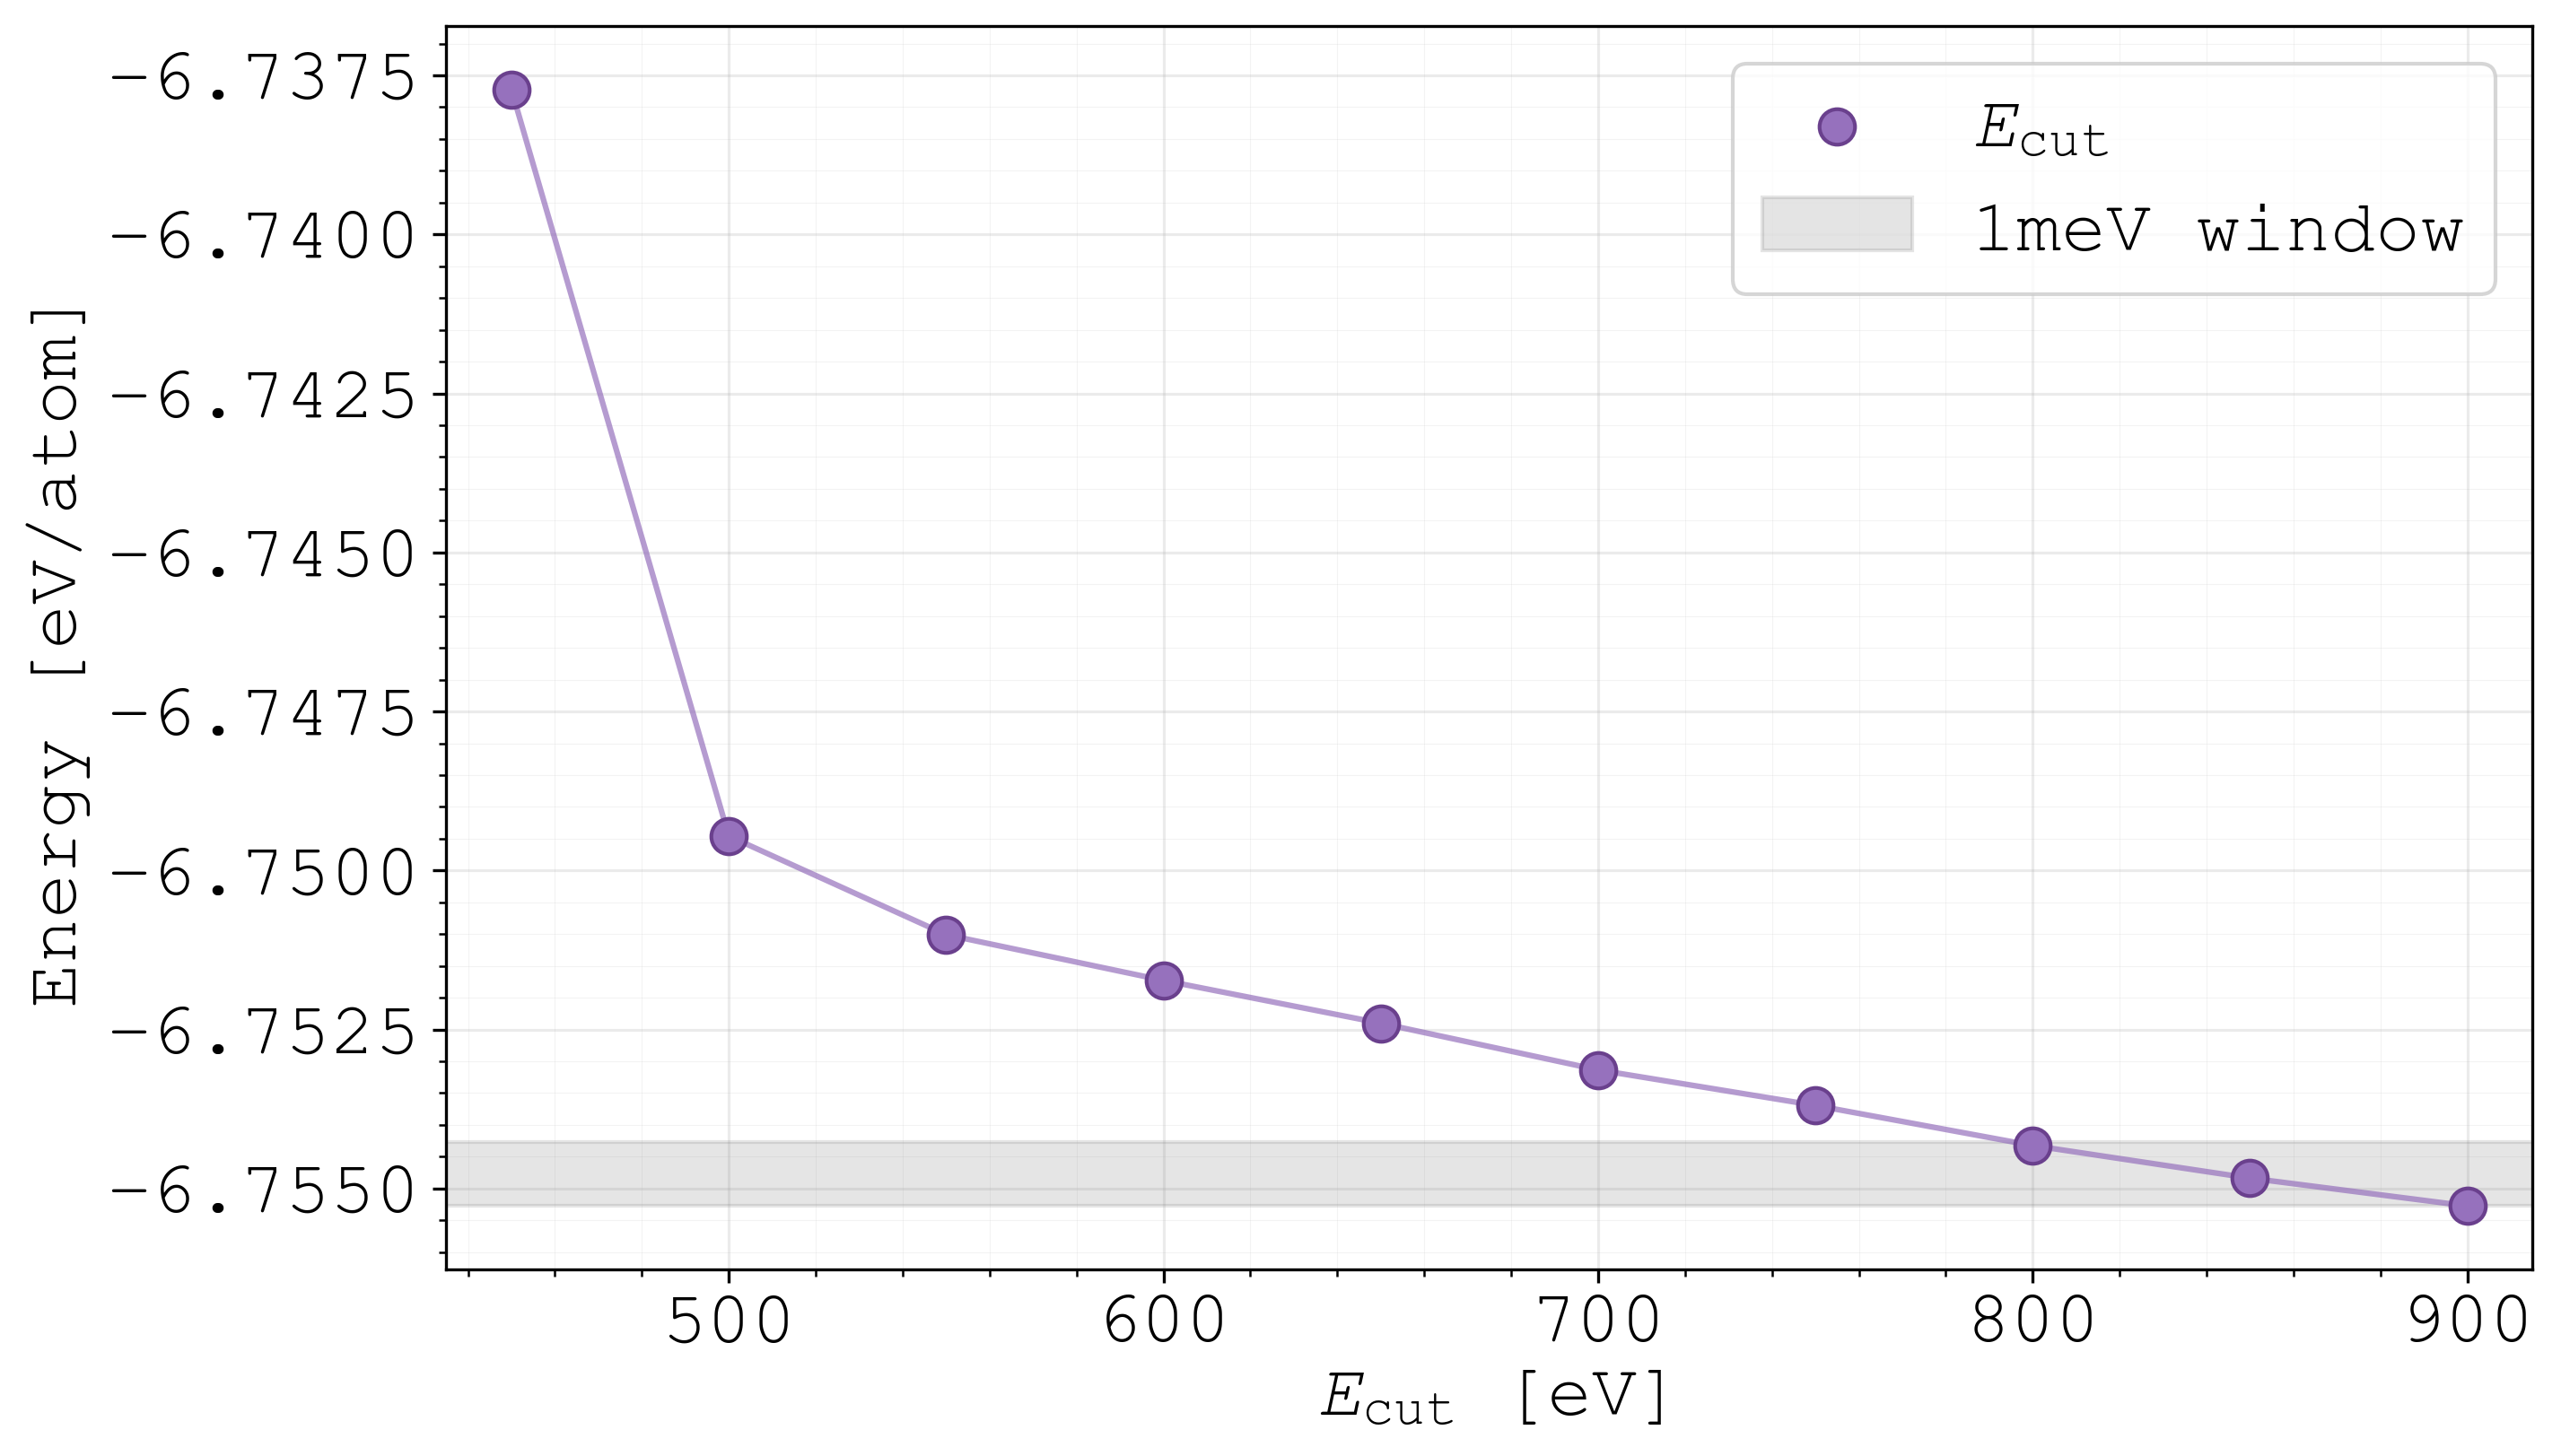
\includegraphics[width=0.8\textwidth]{cutoff-vasp.png}
    \caption{
    Cut-off energy convergence test performed in VASP employing the PBEsol functional for $300 \leq E_{\text{cut}} \leq 900$ eV. The $\Delta E = 1$meV/atom convergence criteria is achieved at $E_{\text {cut}} = 800$ eV}
    \label{cutoff-energy}
\end{figure}

\subsection{k-point convergence}
 Two k-point convergence tests were performed: the first before the initial relaxation of the CSH structure using DFTB+ (GFN1-xTB method), and the second one prior to the full relaxation in VASP (PBEsol functional). In both cases, the convergence criteria of $\Delta E = 1$meV/atom was satisfied with a $\Gamma$-centered ($1\times 1\times 1$) mesh, corresponding to a k-point spacing of $\Delta k=0.06$ Å$^{-1}$ (Figure \ref{dftb-kpoints} and \ref{kpoints-vasp}). 
\begin{figure}[H]
    \centering
    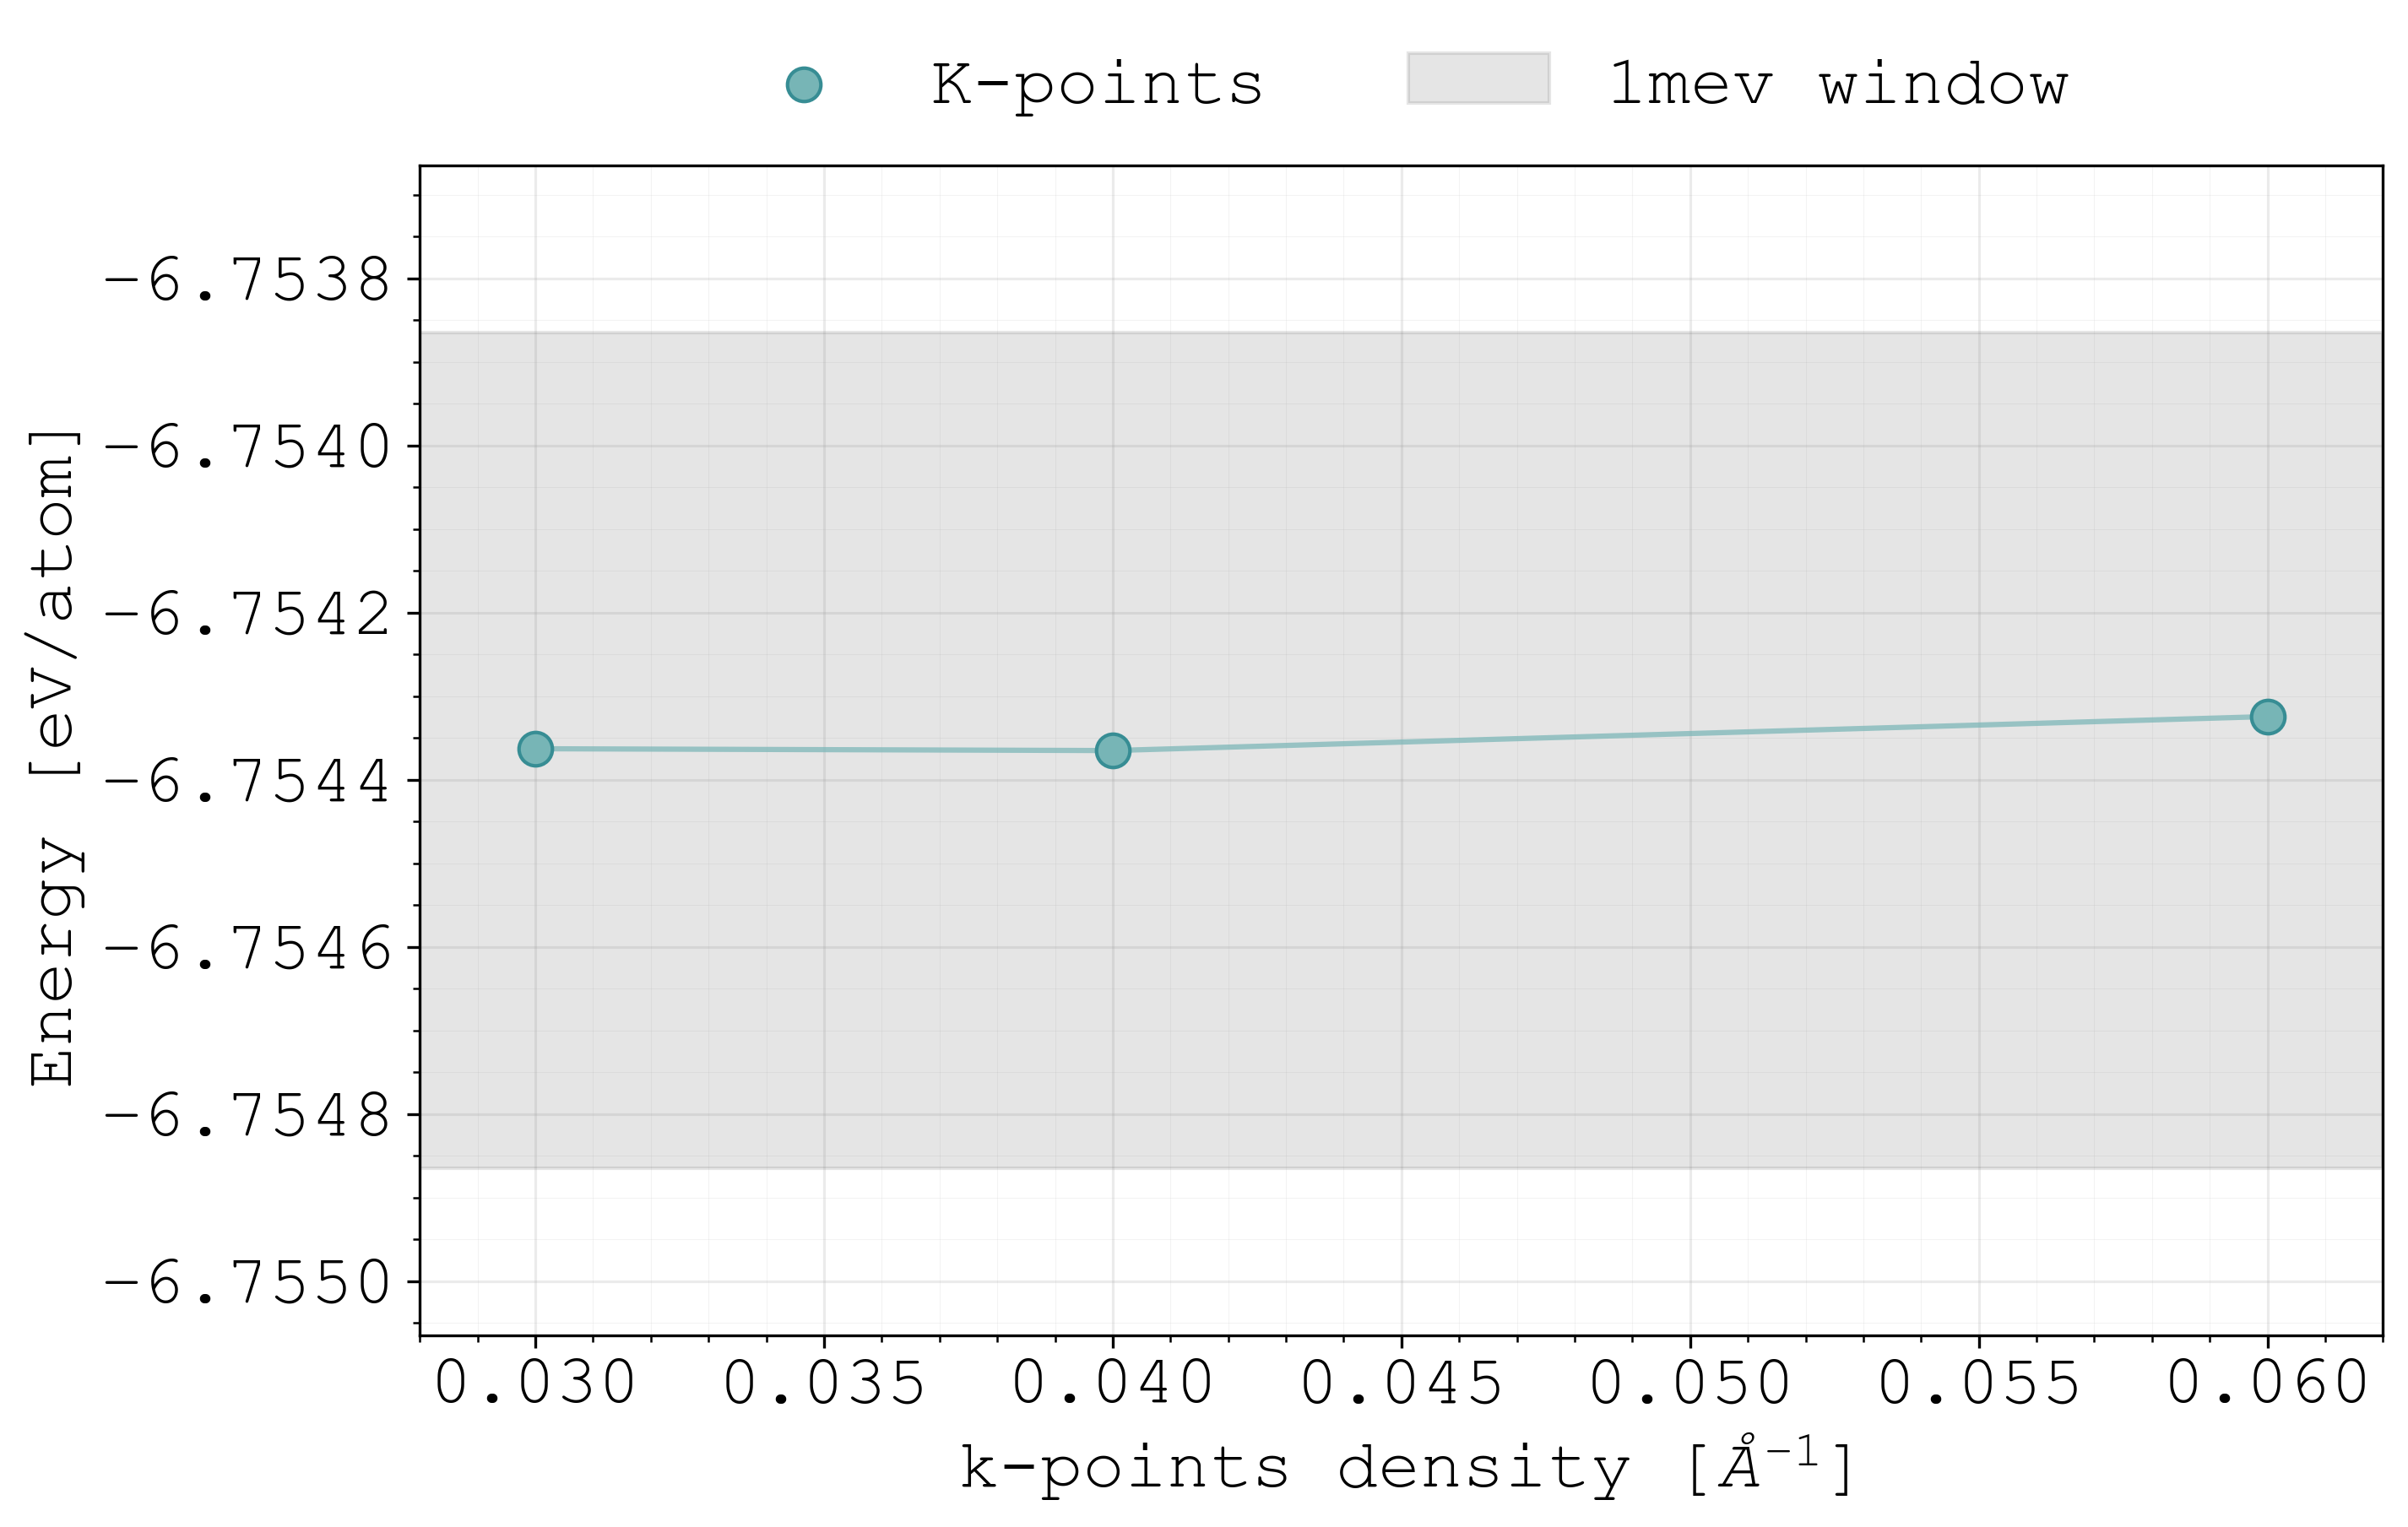
\includegraphics[width=0.8\textwidth]{dftb-kpoints.png}
    \caption{k-point convergence test performed in DFTB+ using the GFN1-xTB method for $0.03 \leq \Delta k \leq 0.06$. The 
    $\Delta E = 1$meV/atom convergence criteria is achieved at  corresponding to a $(1\times 1\times 1)$ k-point grid. 
    }
    \label{dftb-kpoints}
\end{figure}

\begin{figure}[H]
    \centering
    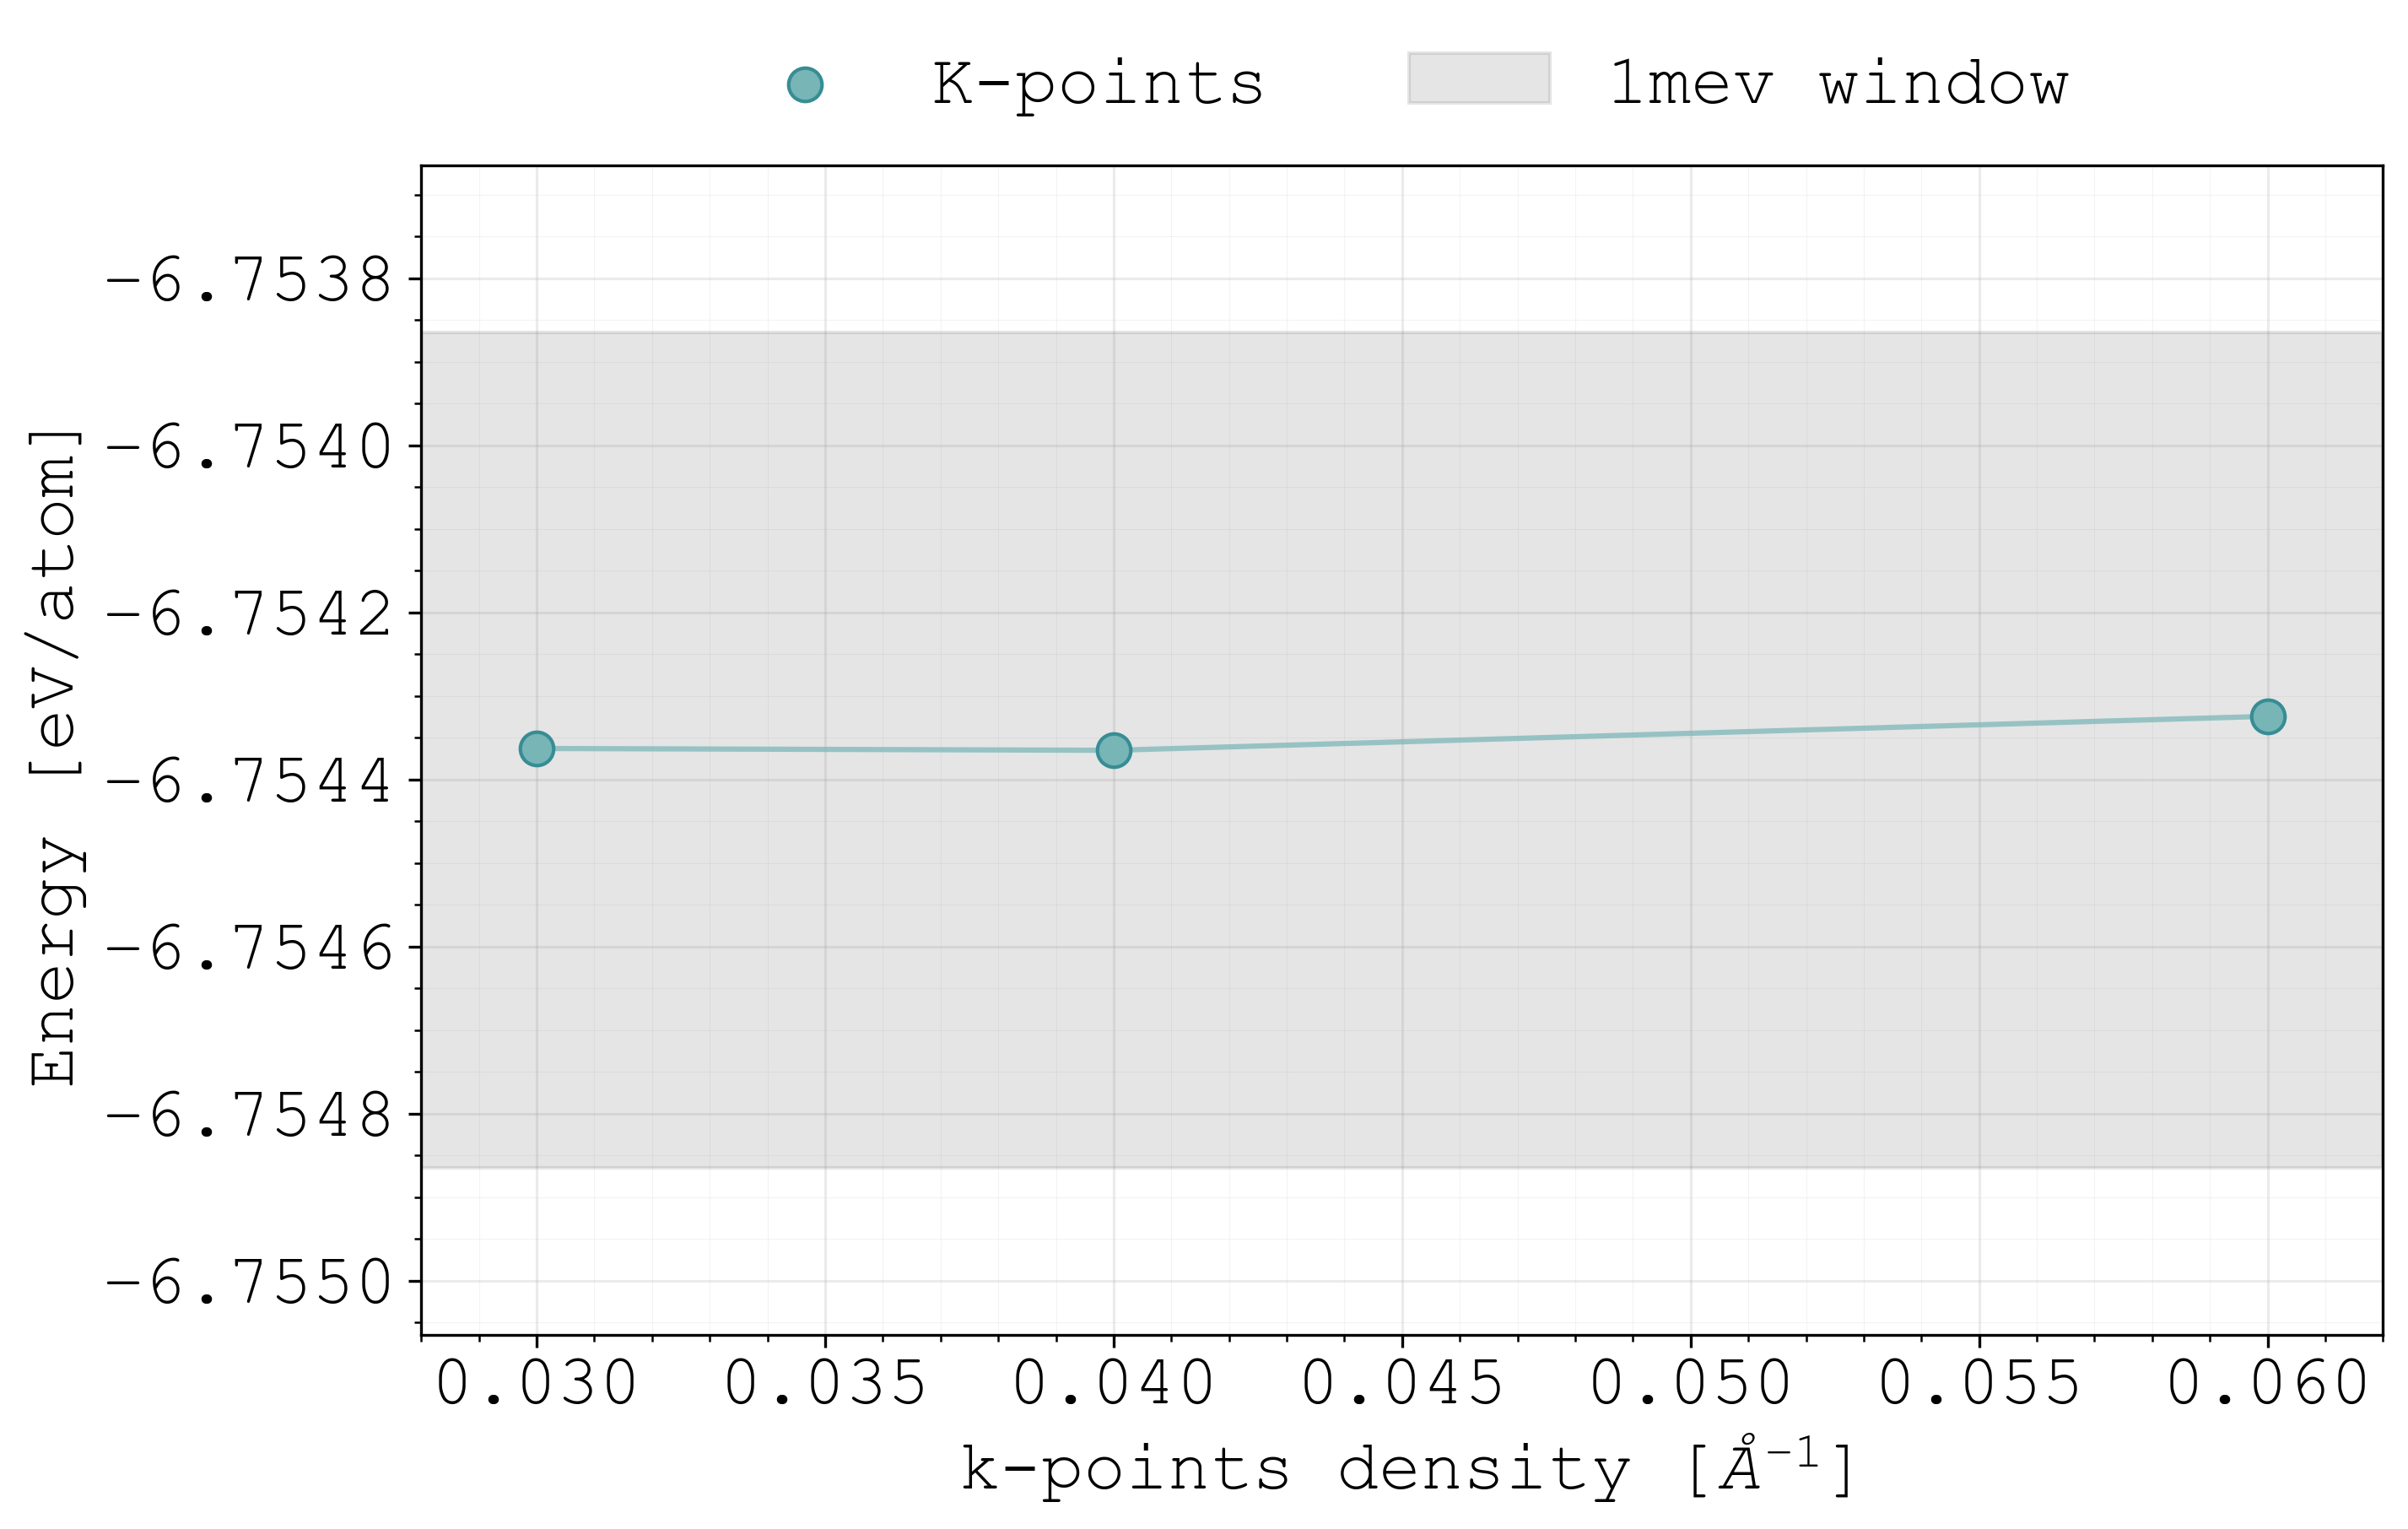
\includegraphics[width=0.8\textwidth]{kpoints-vasp.png}
    \caption{k-point convergence test performed in VASP using the PBEsol functional for $0.03 \leq \Delta k \leq 0.06$. The $\Delta E = 1$meV/atom convergence criteria is achieved at $\Delta k = 0.06 \,\text{\AA}^{-1}$ corresponding to a $(1\times 1\times 1)$ k-point grid, in agreement with the DFTB+ results.
    }
    \label{kpoints-vasp}
\end{figure}
The coarse mesh is justified by the large simulation cell of CSH (690 atoms), which results in a small Brillouin zone, where fine sampling offers no significant improvement to the total energy accuracy\supercite{Kresse1996}.The consistency between DFTB+ and VASP supports the reliability of our choice.  
\subsection{Density of States (DOS)}
The electronic Density of States (DOS) of CSH was calculated using the PBEsol functional in VASP, with the relaxed structure obtained from the optimised cut-off energy and k-point mesh. The resulting DOS are presented in Figure \ref{dos}.

The DOS profile exhibits a clear band gap of approximately 3.0 eV between the valence and conduction bands, with no electronic states in the Fermi level region. The absence of electronic states at $E_F$ confirms the insulating nature of CSH, consistent with its classification as a ceramic material. The valence band is predominantly populated by O2$p$ and Ca3$p$ states, while the conduction band is mainly composed of Ca3$d$ states in fair aggrement with previous computational studies\supercite{Dharmawardhana2018}. 
\begin{figure}[H]
    \centering
    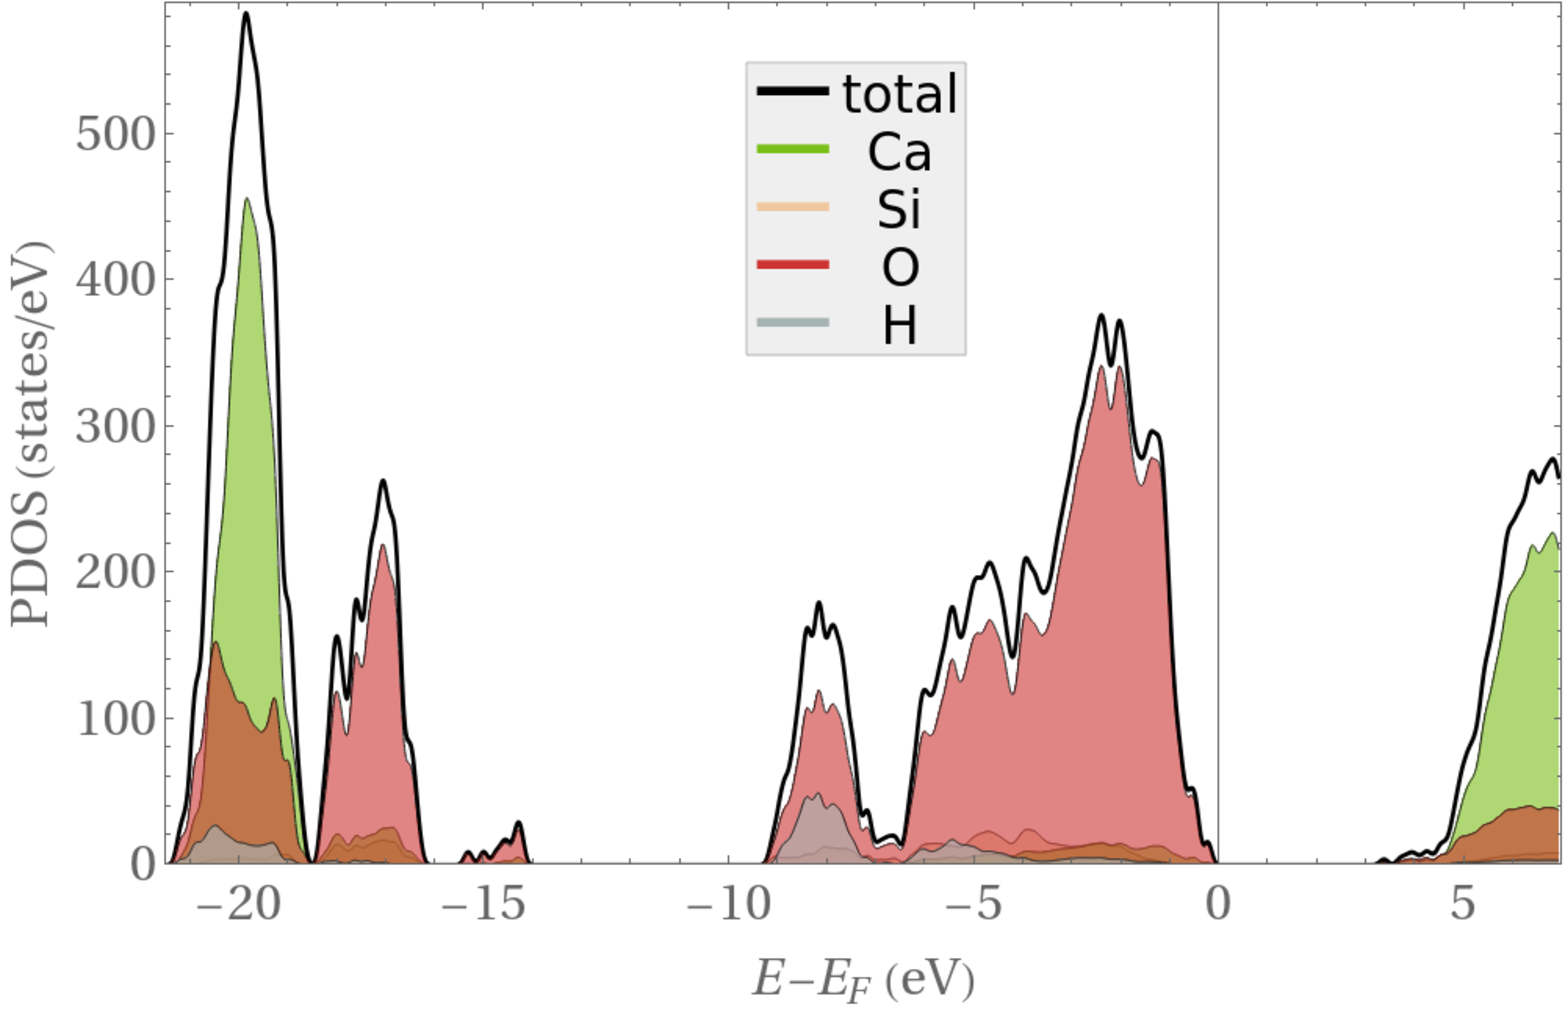
\includegraphics[width=0.7\textwidth]{DOS.pdf}
    \caption{
        Electronic Density of States (DOS) of CSH calculated using the PBEsol functional in VASP after full structure relaxation. Fermi level is set to 0 eV, and a band gap of approximately 3.0 eV is observed. 
    }
    \label{dos}
\end{figure}

\section{Machine Learning Force Field (MLFF) Generation}
\label{sec:mlff-training}

This section is devoted to the core focus of this work, the training,  test and refinement of a machine learning force field (MLFF) for CSH. The MLFF was generated on-the-fly within VASP---which employs a Bayesian-learning algorithm to construct a force field on-the-fly during an AIMD simulation\supercite{zotero-item-773}. We hereby present the training and testing statistics, as well as the details of the final refined MLFF. 
\subsection{Training}
The training phase of the force field consisted of an AIMD simulation performed in VASP using the PBEsol functional, with a time step of 2 fs for a total of 50000 steps (100 ps). Total energy, cell volume and Bayesian error were monitored during the simulation and are reported in Figure \ref{training-stats}. Initial peaks are observed for all three quantities, primarily due to the thermalisation of the~system.

After 10 ps, the total energy stabilises around -4830 eV, with regural fluctuations associated to a increased uncertainty in the force field, whereas the cell volume oscillates around 7500 \AA$^3$. On the other hand, the Bayesian error exhibits a general decreasing trend, reflecting the progressive improvement of the force field as more configurations are explored and added to the training set. Regular spikes in the Bayesian error indicate the appearance of configurations that differ substantially from those previously explored. This prompts the algorithm to switch from prediction to training mode, and the newly identified representative configurations are incorporated into the training set. 
\begin{figure}[H]
    \centering
    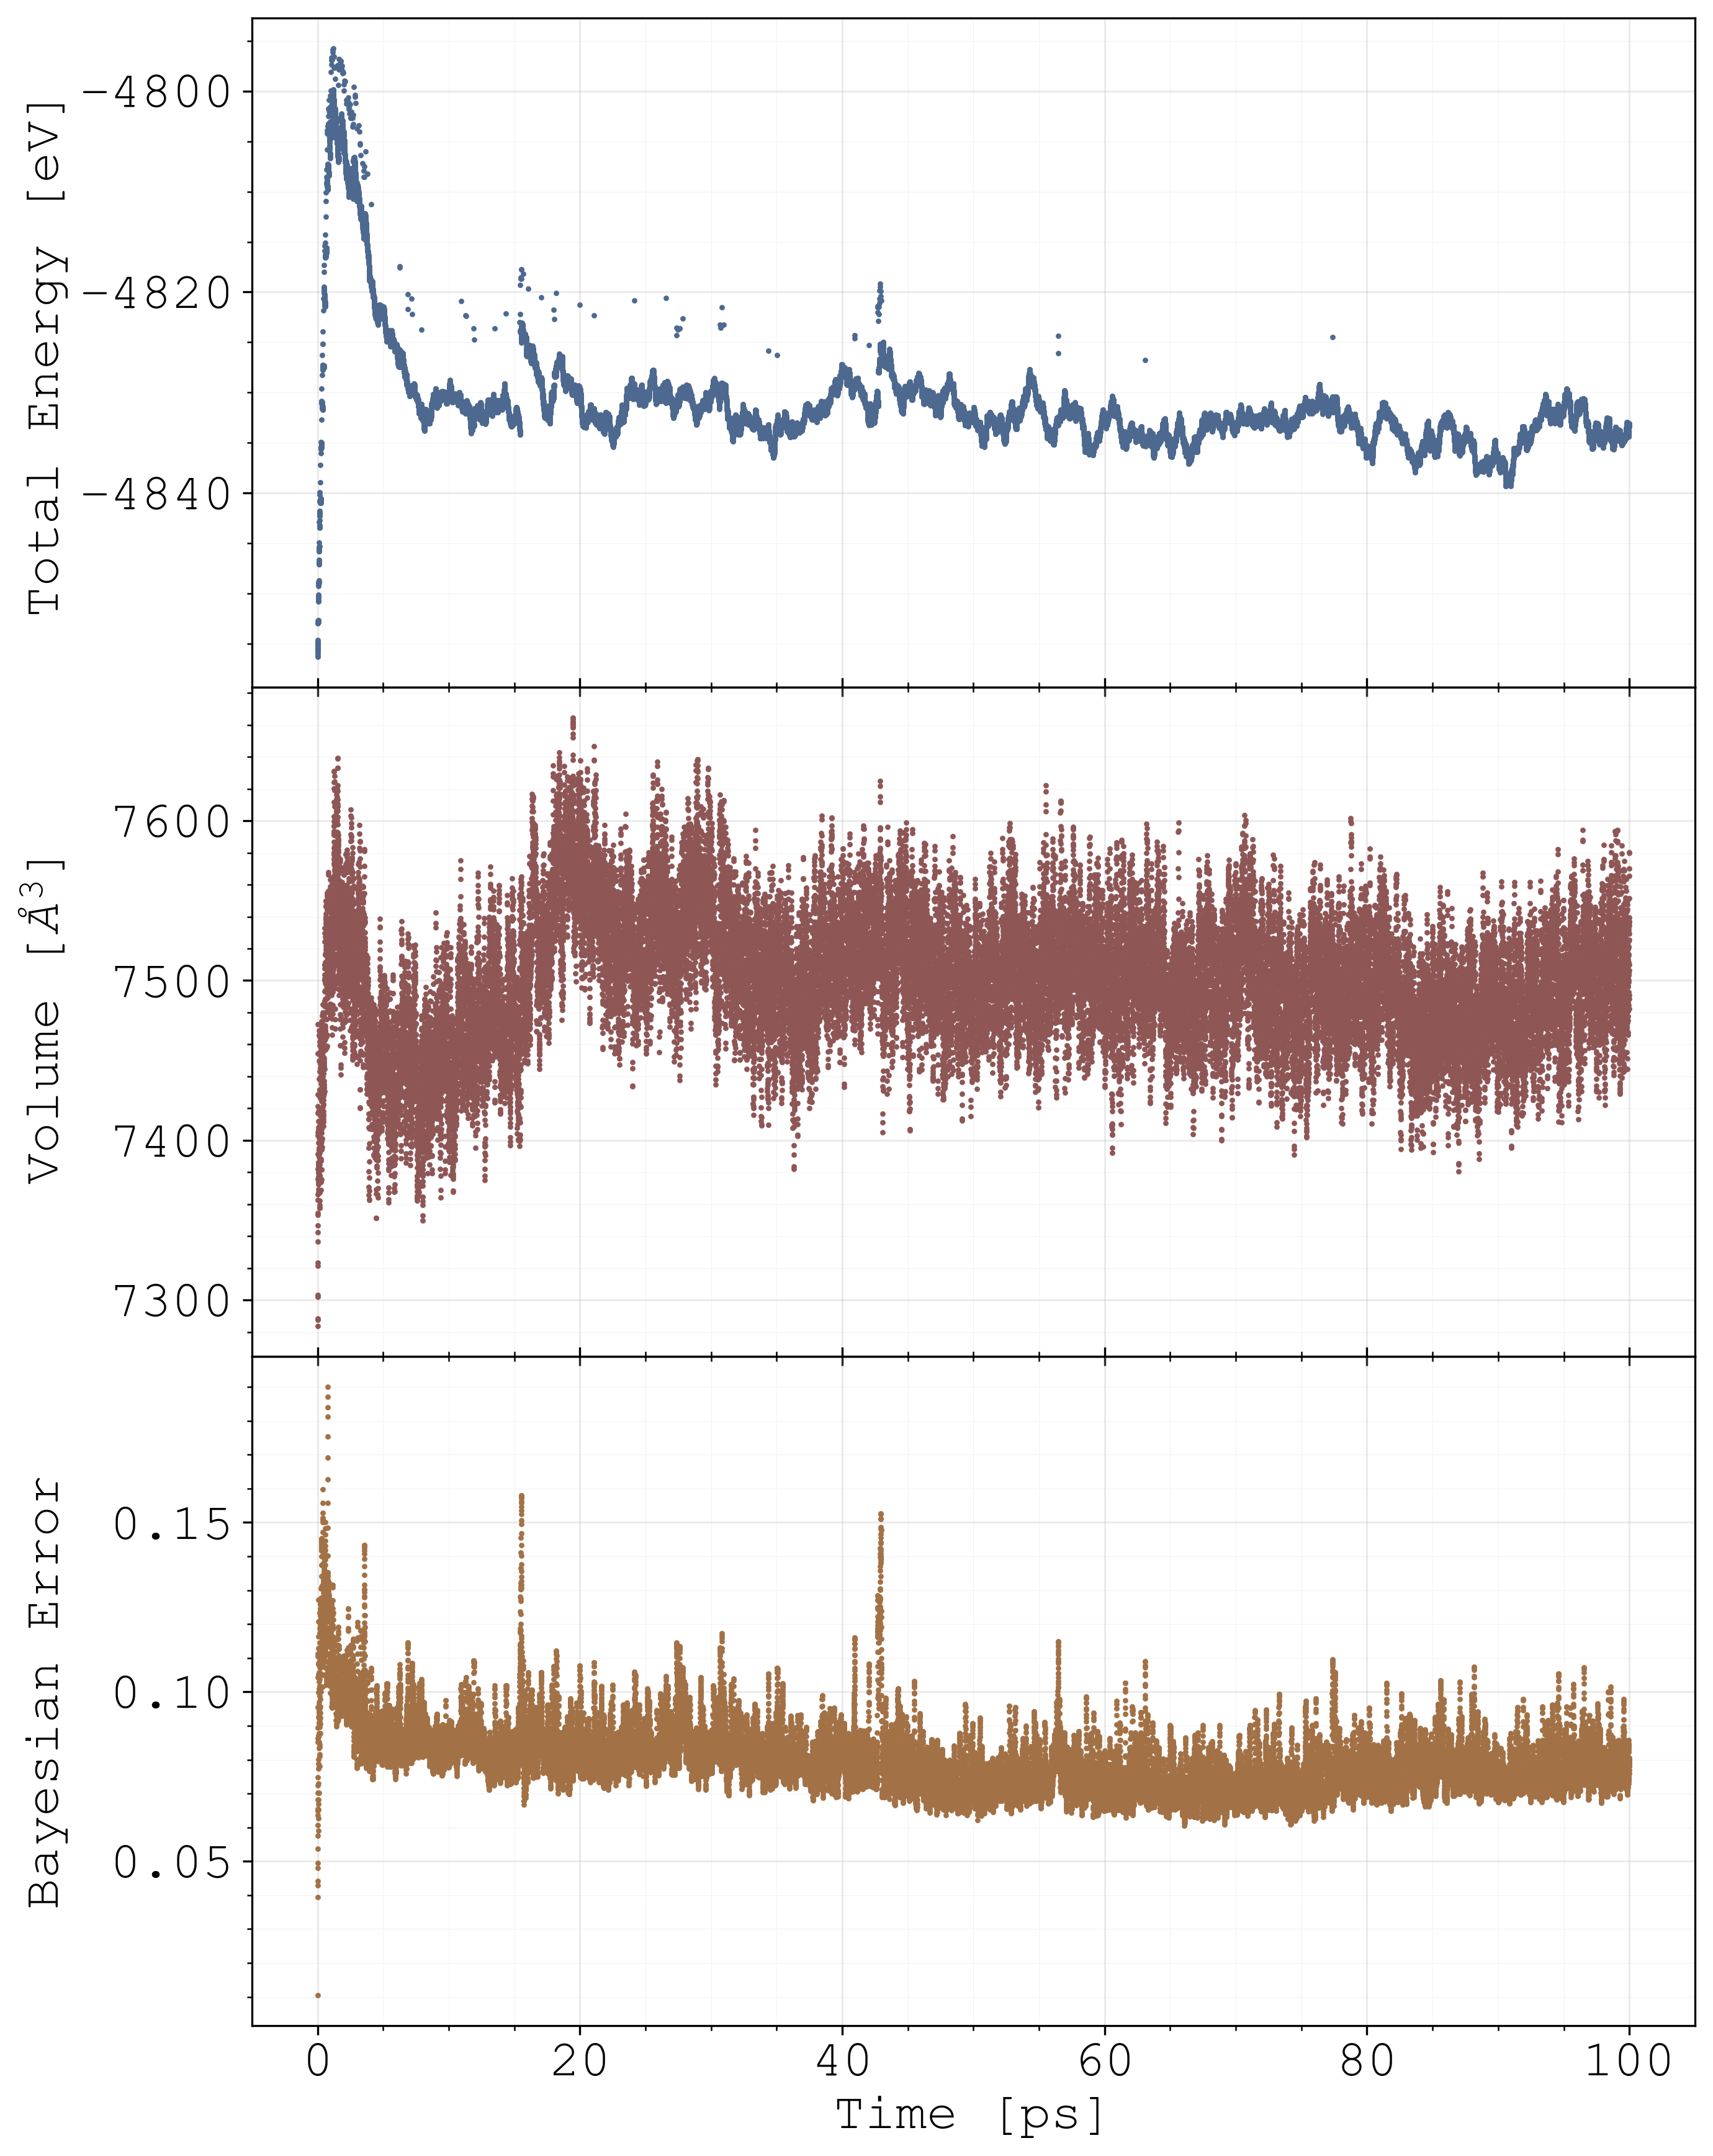
\includegraphics[width=0.8\textwidth]{training-stats.png}
    \caption{
    Training statistics of the MLFF generated on-the-fly during an AIMD simulation in VASP. The plots show the evolution of the total energy, cell volume and the Bayesian error over a total simulation time of 100 ps. 
    }
    \label{training-stats}
\end{figure}

After 80 ps, we observe no significant fluctuations in the total enery, indicating that the force field has converged to a stable representation of the CSH system, as supported by the low Bayesian error. Notably, the final 20 ps of the simulation were performed entirely by the force field in prediction mode, further confirming the stability and reliability of the MLFF.

\subsection{Evaluation}
Following the training phase, we evaluated the performance of the force field in two steps. First, we carried out a MD simulation using the MLFF in prediction mode with a time step of 2 fs for a total simulation time of 100 ps. Second, we randomly selected 50 configurations from the generated trayectory and computed the total energy, forces and stress tensor using both DFT and the MLFF separately. We then computed the errors between the results obtained to quantify the performance of the force field. 

Figure \ref{pred-stats} shows the evolution of the total energy and the cell volume during the MD simulation in prediction mode. No abrupt fluctuations or drifts are observed, with the total energy oscillating aroung -4833 eV and the cell volume around 7494 \AA$^3$. These results show consistency with the training statistics, and reflect the ability of the MLFF to accurately represent the potential energy surface of CSH. 
\begin{figure}[h!]
    \centering
    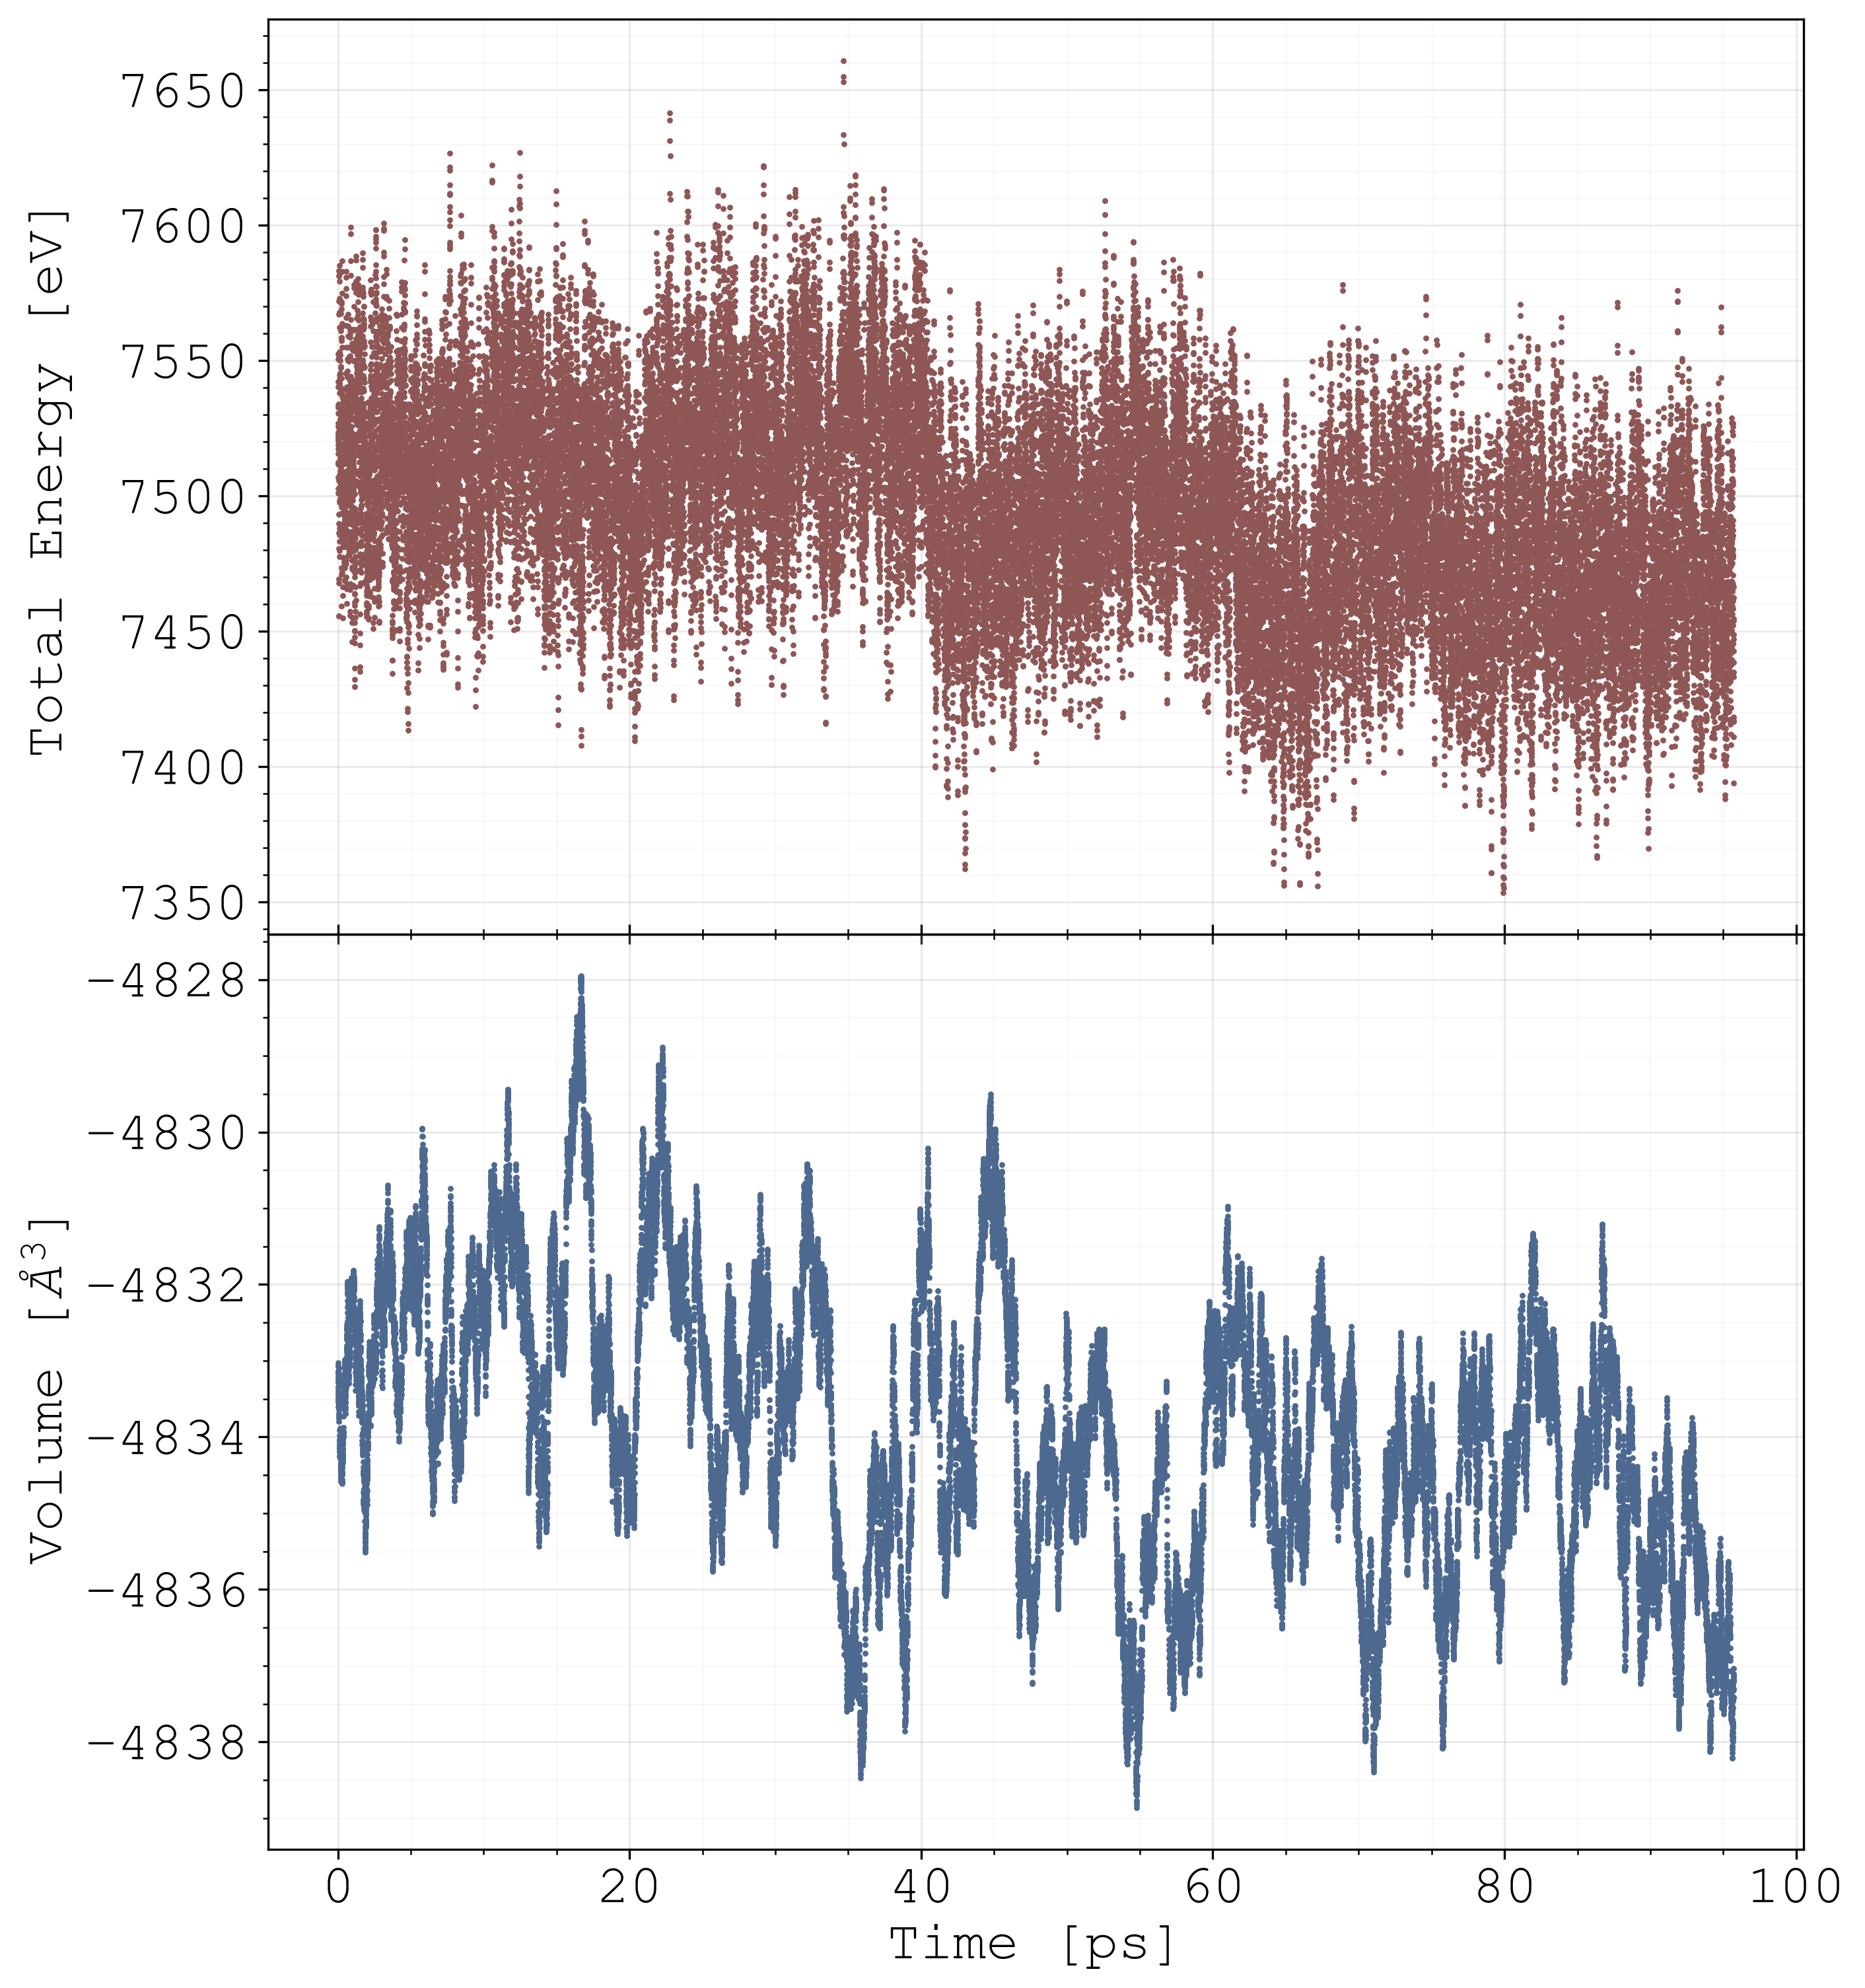
\includegraphics[width=0.8\textwidth]{pred-stats.png}
    \caption{
    Evolution of the total energy and cell volume during a MD simulation of CSH using the MLFF in prediction mode over a total simulation time of 100 ps.  
    }
    \label{pred-stats}
\end{figure}

On the other hand, the errors between DFT and MLFF predictions for the total energy, forces and stress tensor are reported in Figure \ref{pred-errors}. A mean absolute error (MAE) of 12.1 meV/atom is observed for the total energy, and an average root mean square error (RMSE) of 222 meV/Å for the forces and 0.896 kbar for the stress tensor. Similar work on CSH (C/S=1.7) conducted by Zhu \supercite{Zhu2024} reported a mean total energy error of 6 meV/atom and an RMSE of 160 meV/Å for the forces, rendering our MLFF comparable in terms of accuracy. As for the stress tensor RMSE, no avaliable data was found for comparison. Finally, we can further improve the reported errors by refining the MLFF, as discussed in the next subsection.

\begin{figure}[h]
    \centering
    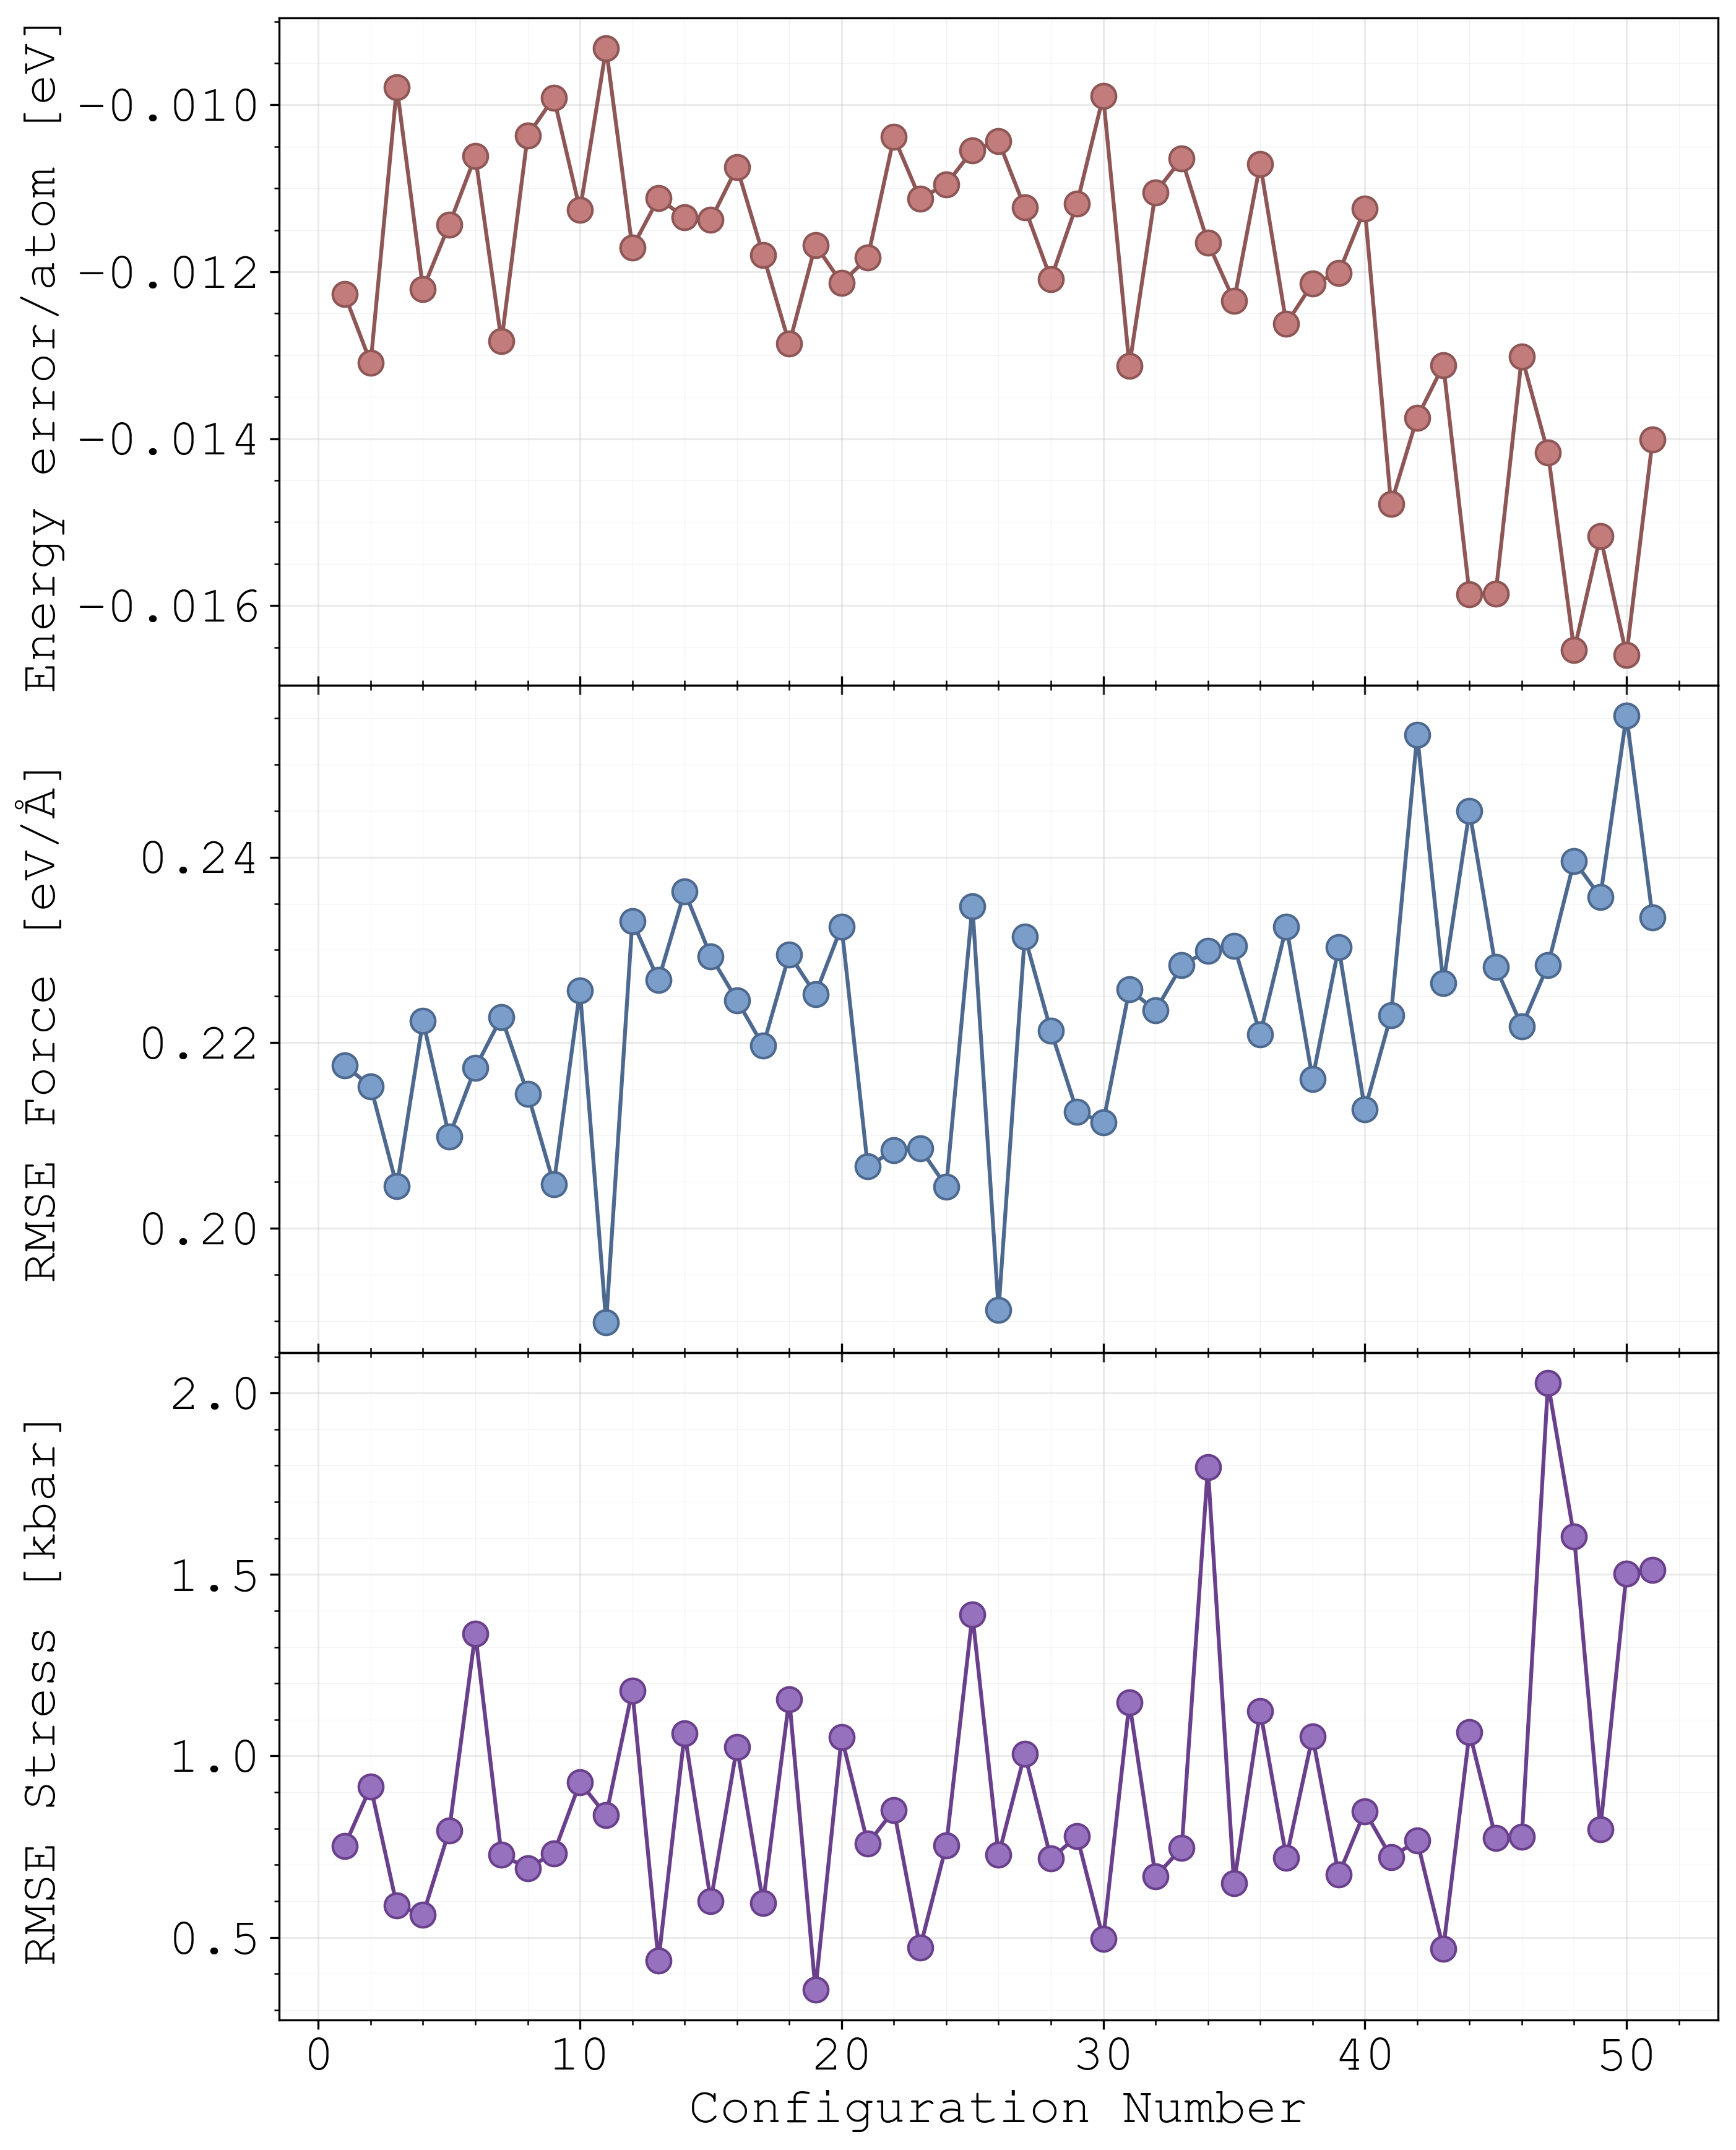
\includegraphics[width=0.8\textwidth]{pred-errors.png}
    \caption{
    Energy error per atom and root mean square error (RMSE) for forces and stress tensor of CSH between DFT and MLFF predictions, evaluated on 50 configurations randomly selected from an independent set of 50000 configurations generated via MD simulation using the MLFF in prediction mode without refiting. 
    }
    \label{pred-errors}
\end{figure}

\subsection{Refinement}
The MLFF refinement involved varying hyperparameters of the force field, running a refitting procedure and evaluating the performance of the refined MLFF. In this work, we focused on the radial and angular descriptors, as they are crucial for the representation of the local interactions of atoms in CSH. Figure \ref{rcut1} and \ref{rcut2} show the error dependence on the radial and angular descriptors, respectively. 

\begin{figure}[h]
    \centering
    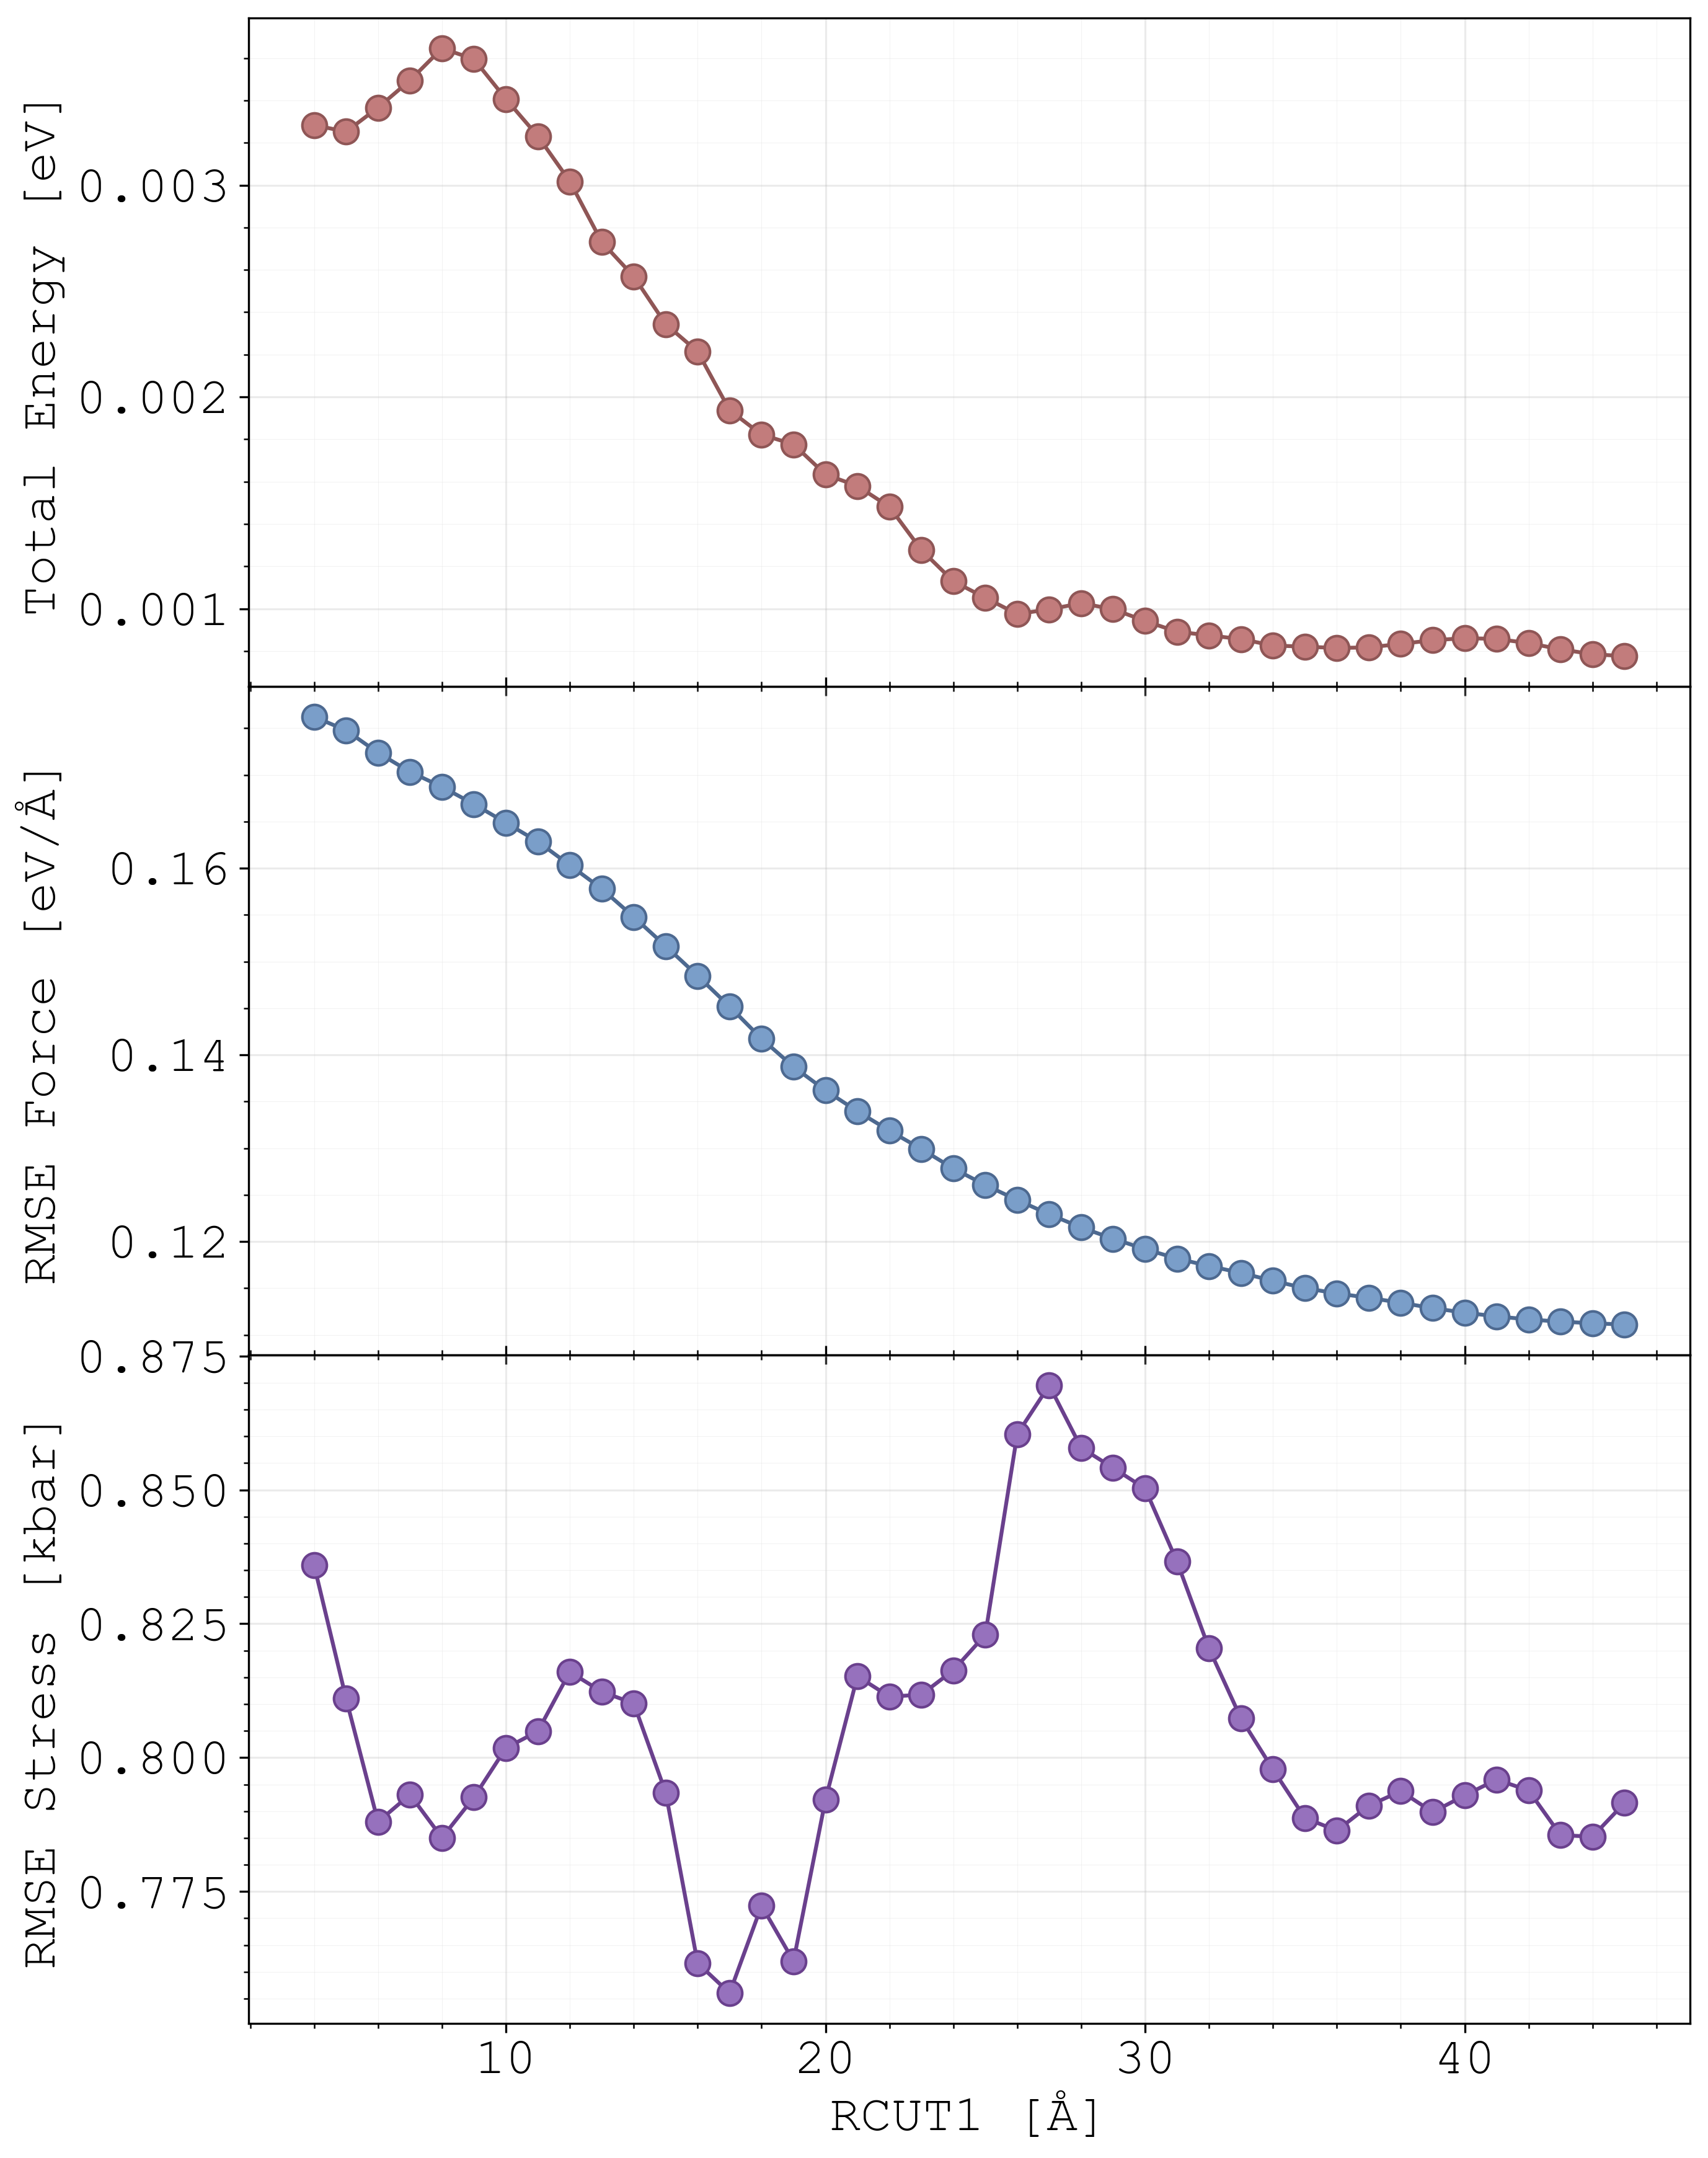
\includegraphics[width=0.8\textwidth]{rcut1.png}
    \caption{
    Root mean square error (RMSE) for the total energy, forces and stress tensor as a function of the radial descriptor (\texttt{RCUT1}). 
    }
    \label{rcut1}
\end{figure}
We varied the radial descriptor (\texttt{RCUT1}) over the range of 4.0 to 45.0 Å, and the angular descriptor (\texttt{RCUT2}) over the range 2.0 to 10.0 Å. With the energy error and the force RMSE monotonically decreasing, no clear minimum is observed for \texttt{RCUT1} in the considered range; however, a minimum stress RMSE occurs at 17.0 \AA. Conversely, \texttt{RCUT2} exhibits a clear minima for both the energy error and the force RMSE at 3.0 \AA, and for the stress tensor RMSE at 4.0 \AA.

\begin{figure}[h]
    \centering
    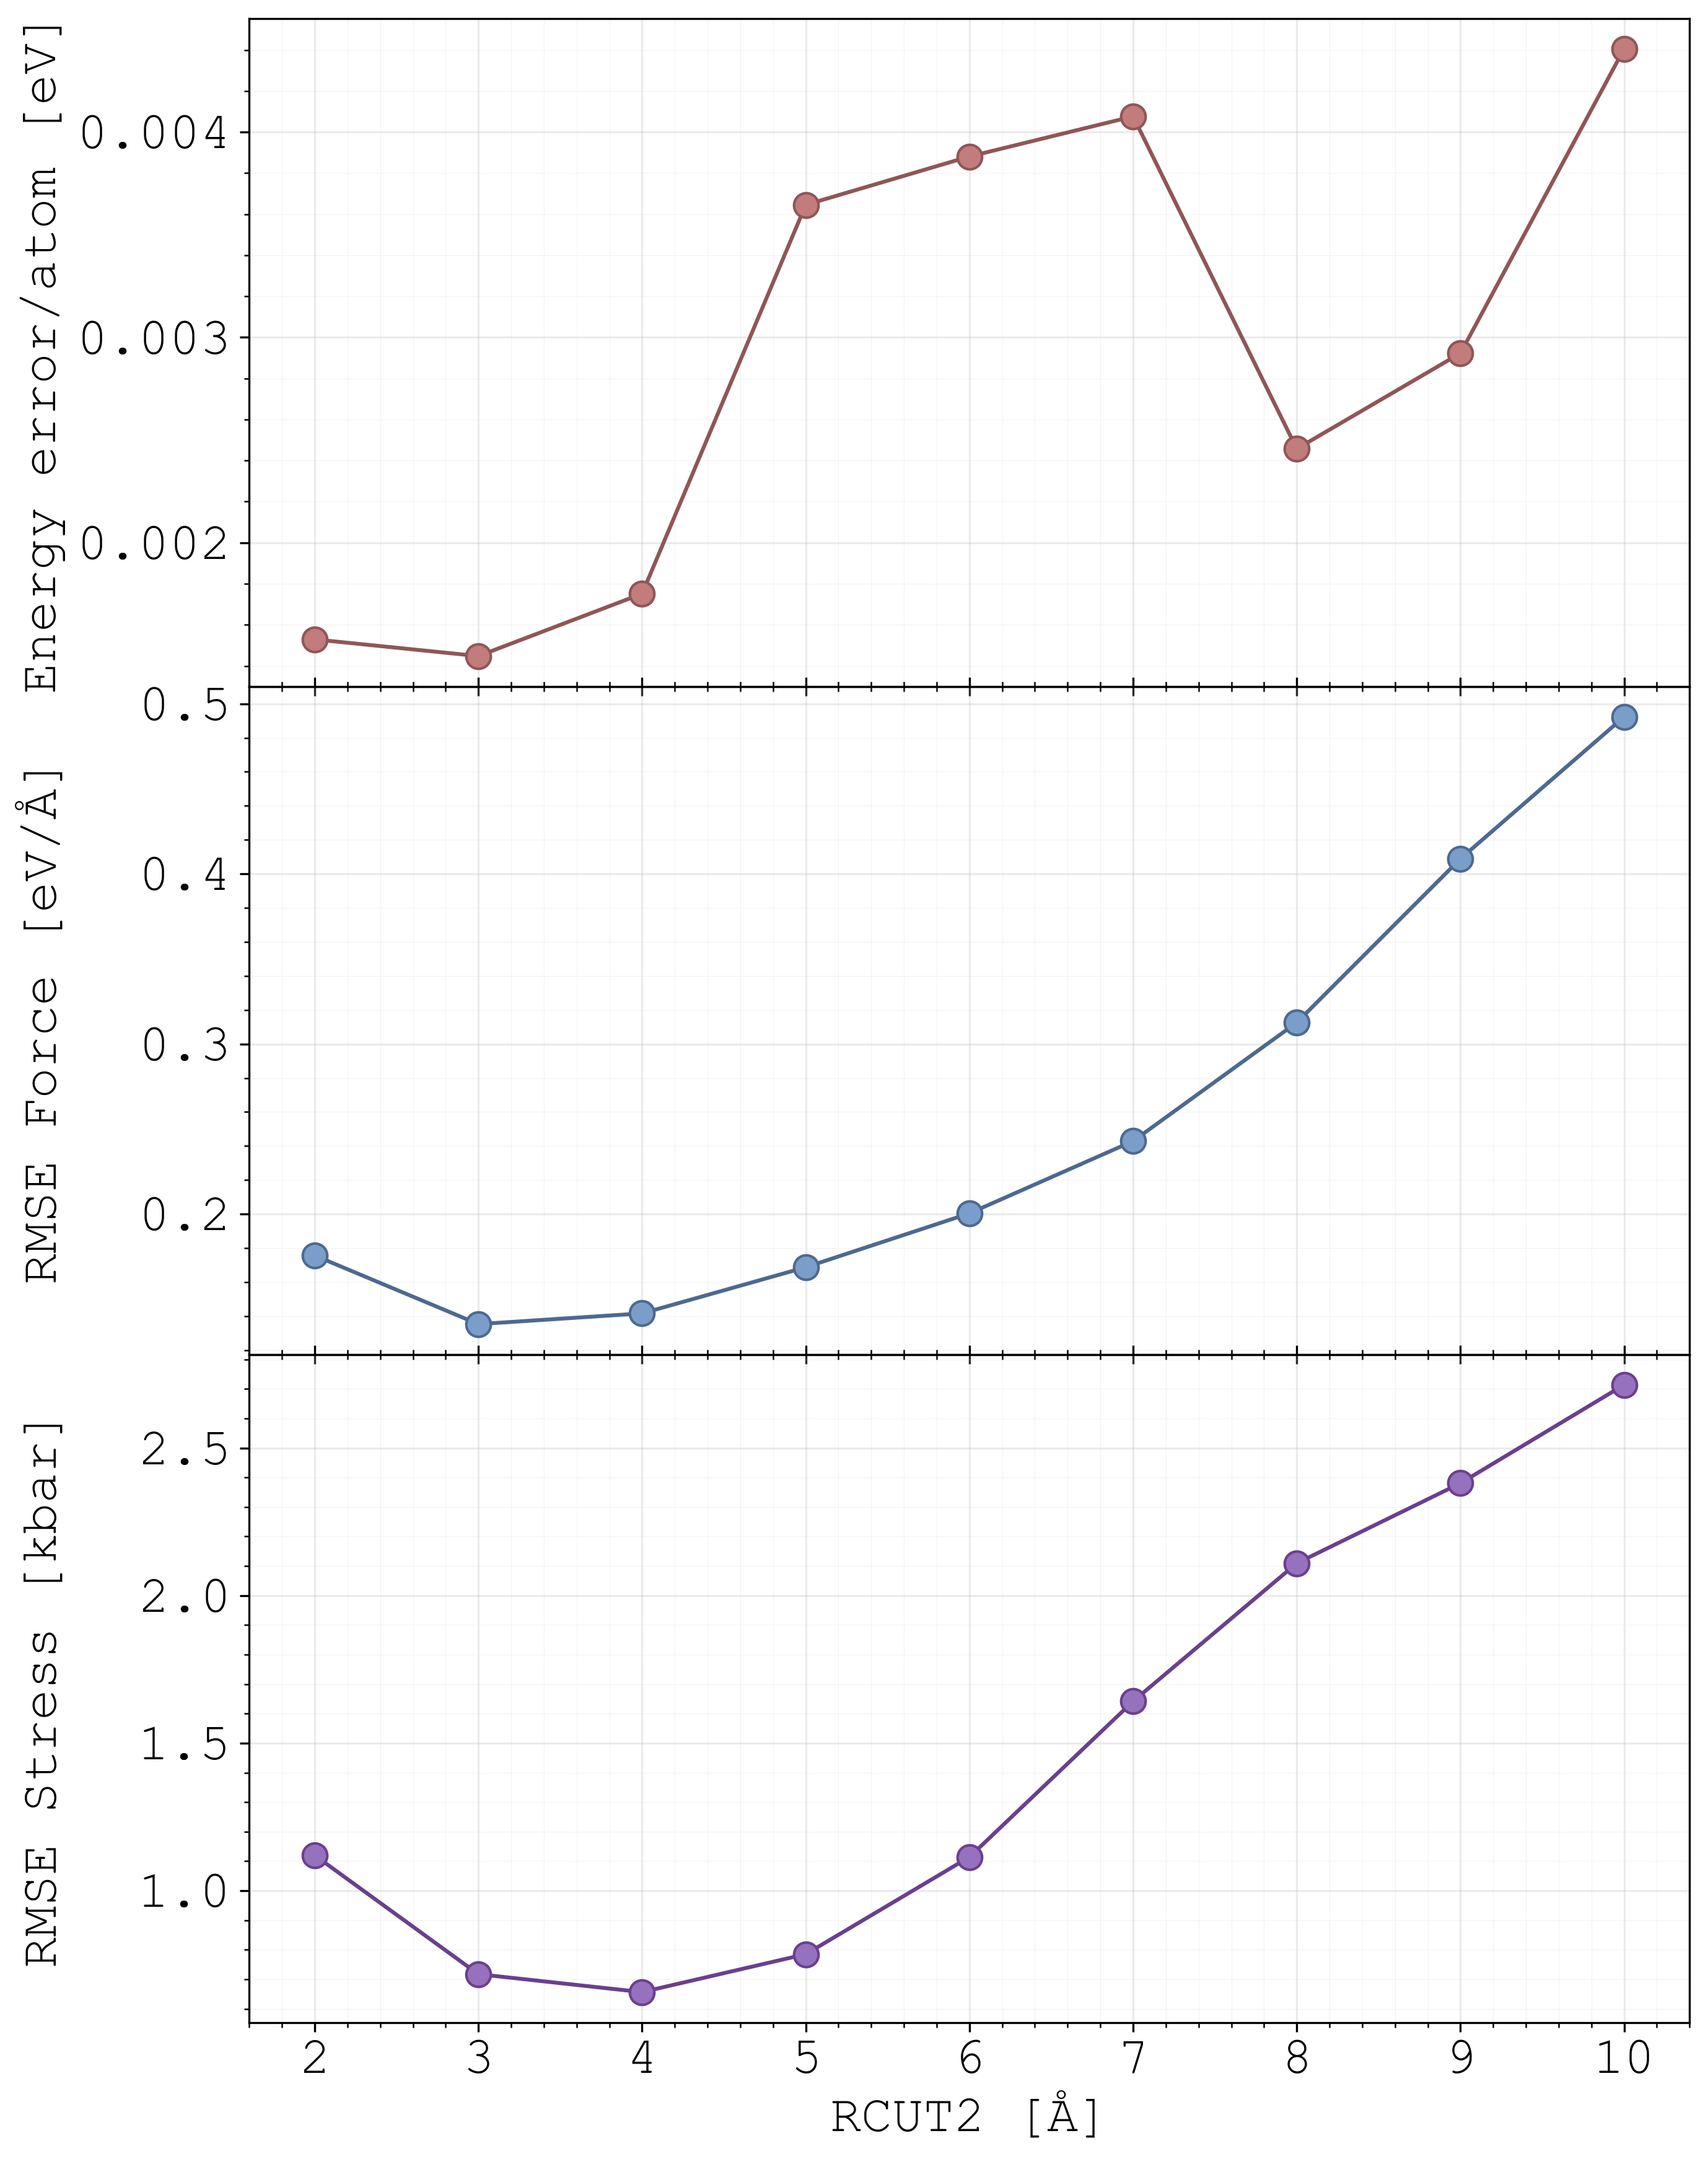
\includegraphics[width=0.8\textwidth]{rcut2.png}
    \caption{
    Root mean square error (RMSE) for the total energy, forces and stress tensor as a function of the angular descriptor (\texttt{RCUT2}).
    }
    \label{rcut2}
\end{figure}

Based on these results, two refined MLFFs were generated: \textbf{FF1} with \texttt{RCUT1}=17.0 Å and \texttt{RCUT2}=4.0 Å, and \textbf{FF2} with \texttt{RCUT1}=36.0 Å and \texttt{RCUT2}=4.0 Å. Additionally, we called \textbf{FF0} the original MLFF generated during the training phase, which used \texttt{RCUT1}=5.0 Å and \texttt{RCUT2}=6.0~Å. \textbf{FF2} was chosen to explore the effect of a larger radial descriptor, albeit no performance evaluation was carried out due to the computational cost. 
The performance of \textbf{FF1} was evaluated following the same procedure as before, and the results are presented in Figure \ref{rf-pred-errors}. A significant improvement is observed, with a MAE of  1.039 meV/atom for the total energy and an average RMSE of 163 meV/Å for the forces, whereas the stress tensor RMSE increased to 1.19 kbar.
\begin{figure}[h]
    \centering
    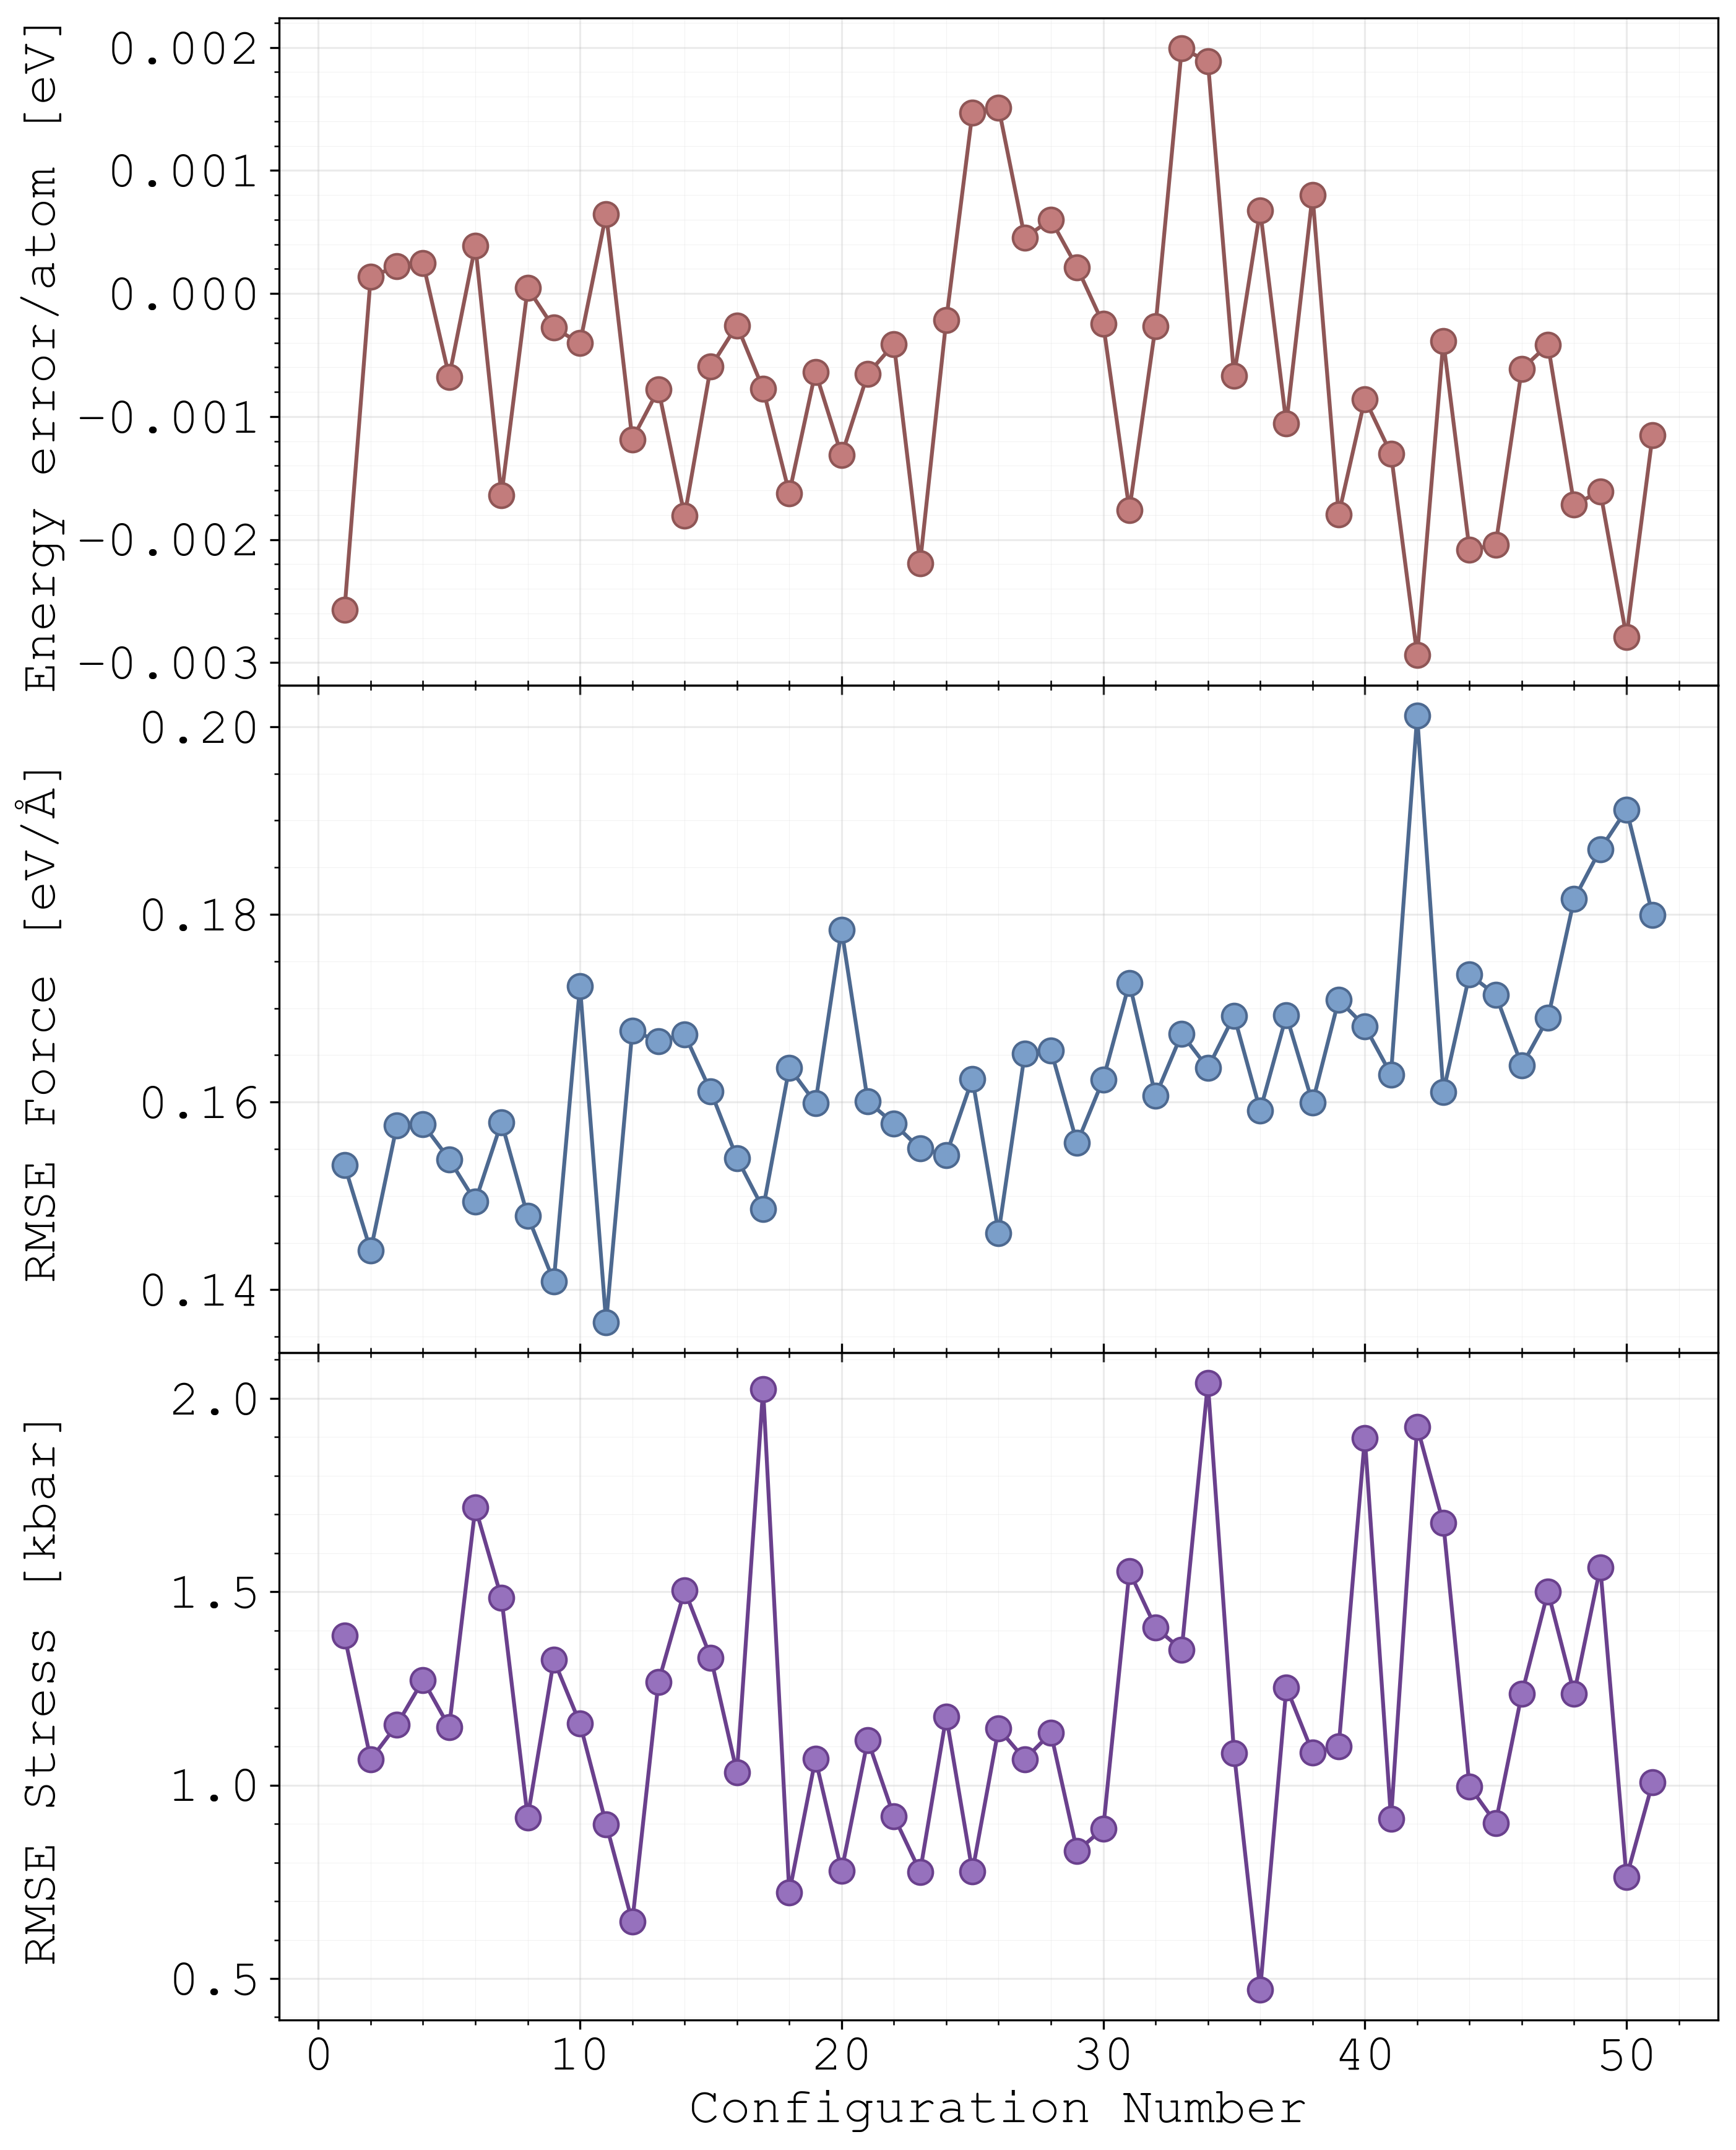
\includegraphics[width=0.8\textwidth]{rf-pred-errors.png}
    \caption{
    Energy error per atom and root mean square error (RMSE) for forces and stress tensor of CSH between DFT and MLFF predictions, evaluated on 50 configurations using the refined MLFF \textbf{FF1}.  
    }
    \label{rf-pred-errors}
\end{figure}
\section{Thermodynamic Properties of CSH}
\label{sec:thermo-properties}
In this section, we present the thermodynamic properties of CSH, including the equation of state (EOS) and optimal bulk parameters. To this end, the three MLFFs generated in the previous section were employed to perform a series of energy-volume calculations and fit the Birch-Murnaghan equation of state (EOS) to the results. Obtained results are summarised in Table \ref{tab:bulk-params}.

\subsection{Equation of State (EOS) and Bulk Parameters}
Figure \ref{fig:eos-ff0}, \ref{fig:eos-ff1} and \ref{fig:eos-ff2} show the Birch-Murnaghan equation of state (EOS) obtained by fitting the enrgy-volume data obtained wuth \textbf{FF0}, \textbf{FF1} and \textbf{FF2}, respectively.  For the three cases we employed the same input strtucture---the relaxed CSH structure obtained in Section \ref{sec:bulk-params-dos}---and performed a series of energy-volume calculations by varying the cell volume within a range of 1\% around the relaxed volume. 


\begin{figure}[h!]
    \centering
    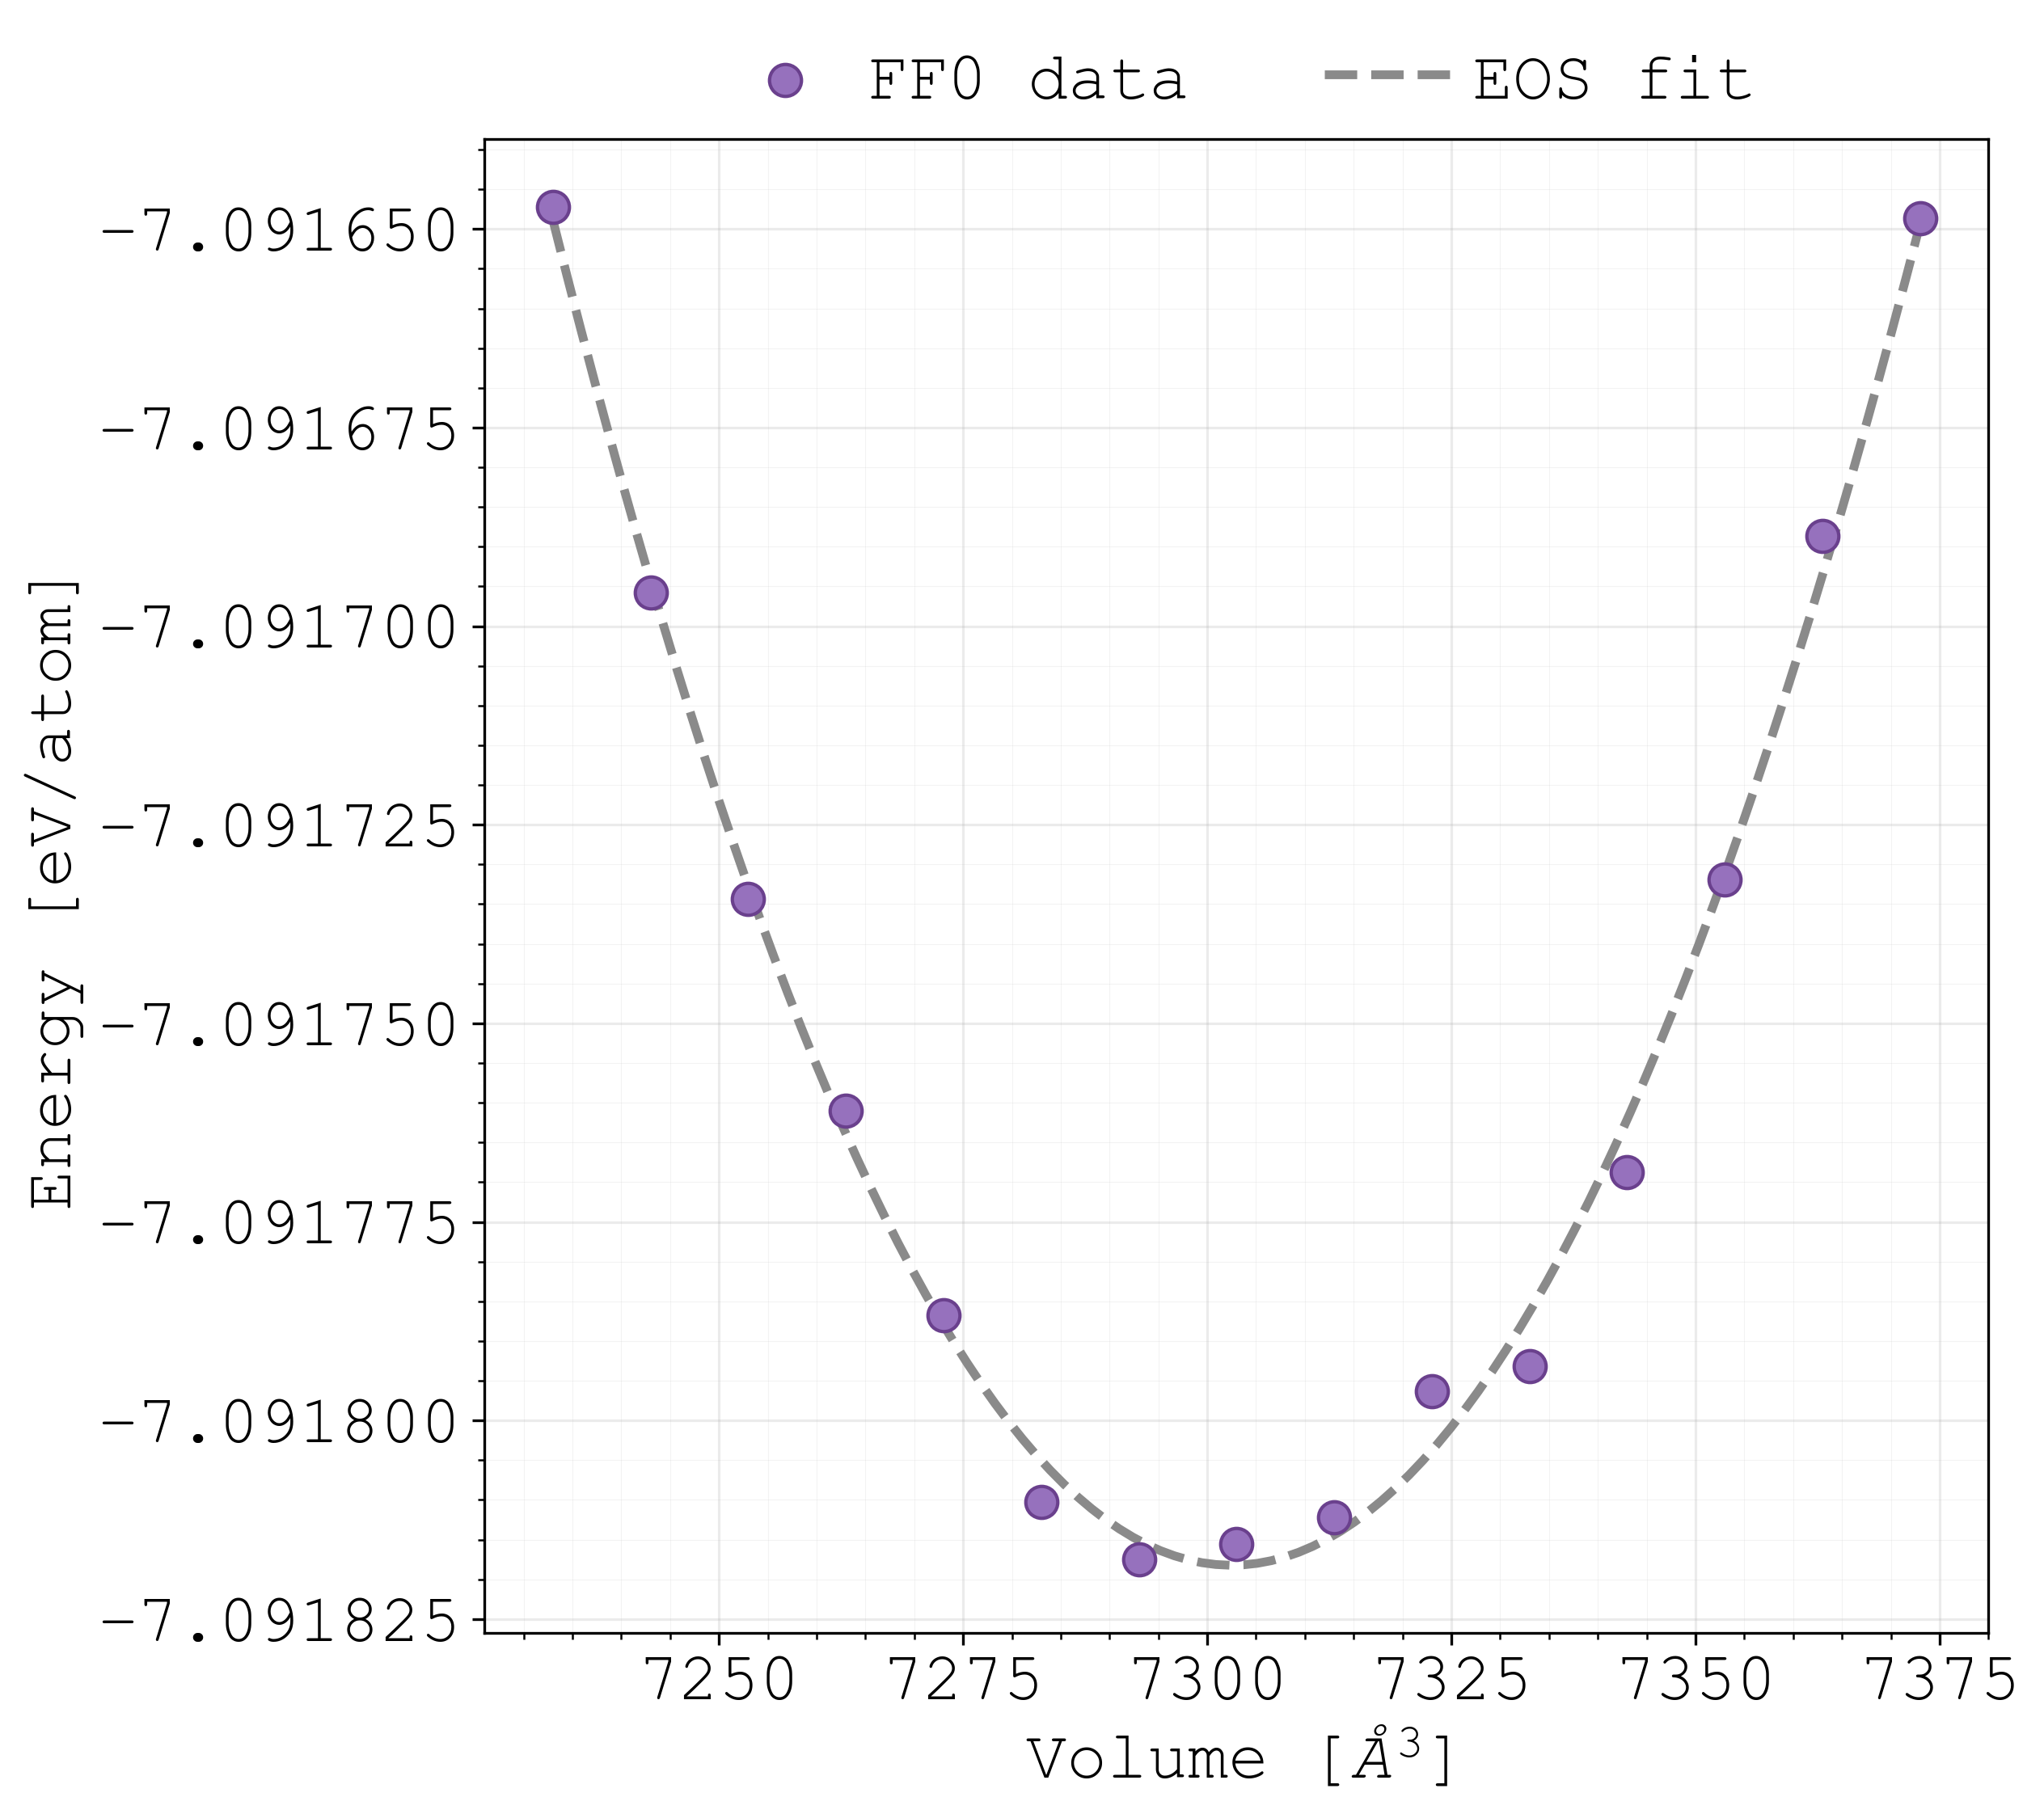
\includegraphics[width=0.7\textwidth]{EOS-FF0.png}
    \caption{Birch-Murnaghan equation of state (EOS) obtained by fitting the energy-volume obtained with \textbf{FF0} (red dots) for CSH. Optimal volume $V_0=7302.49$ \AA$^3$ and bulk modulus $B_0=55.72$ GPa are reported.
    }
    \label{fig:eos-ff0}
\end{figure}

We observe a good agreement in the optimal energy $E_0$ and bulk modulus $B_0$ values obtained with the three models; however, the optimal volume $V_0$ for \textbf{FF2} shows a significant deviation compated to the rest of the models. This can be attributed to the large radial descriptor used in \textbf{FF2}, which may be causing the force field to overfit the training data and not generalise well to the energy-volume relationship. Moreover, the bulk modulus derivative $B_0'$ is negative for \textbf{FF2}, indicating a non-physical behaviour. Thereby, model \textbf{FF2} was not considered for further~analysis. 

Overall, a good agreement is observed between the $B_0$ values obtained with \textbf{FF0} and \textbf{FF1} and the experimental value of $47\pm 3$ GPa reported by Oh \emph{et al.}\supercite{Oh2012}. Additionally, the $B_0'$ parameter obtained with \textbf{FF0} is closer to the experimental value of 4\supercite{Oh2012}, whereas \textbf{FF1} shows a significantly higher value of 9.8. 
\begin{figure}[h!]
    \centering
    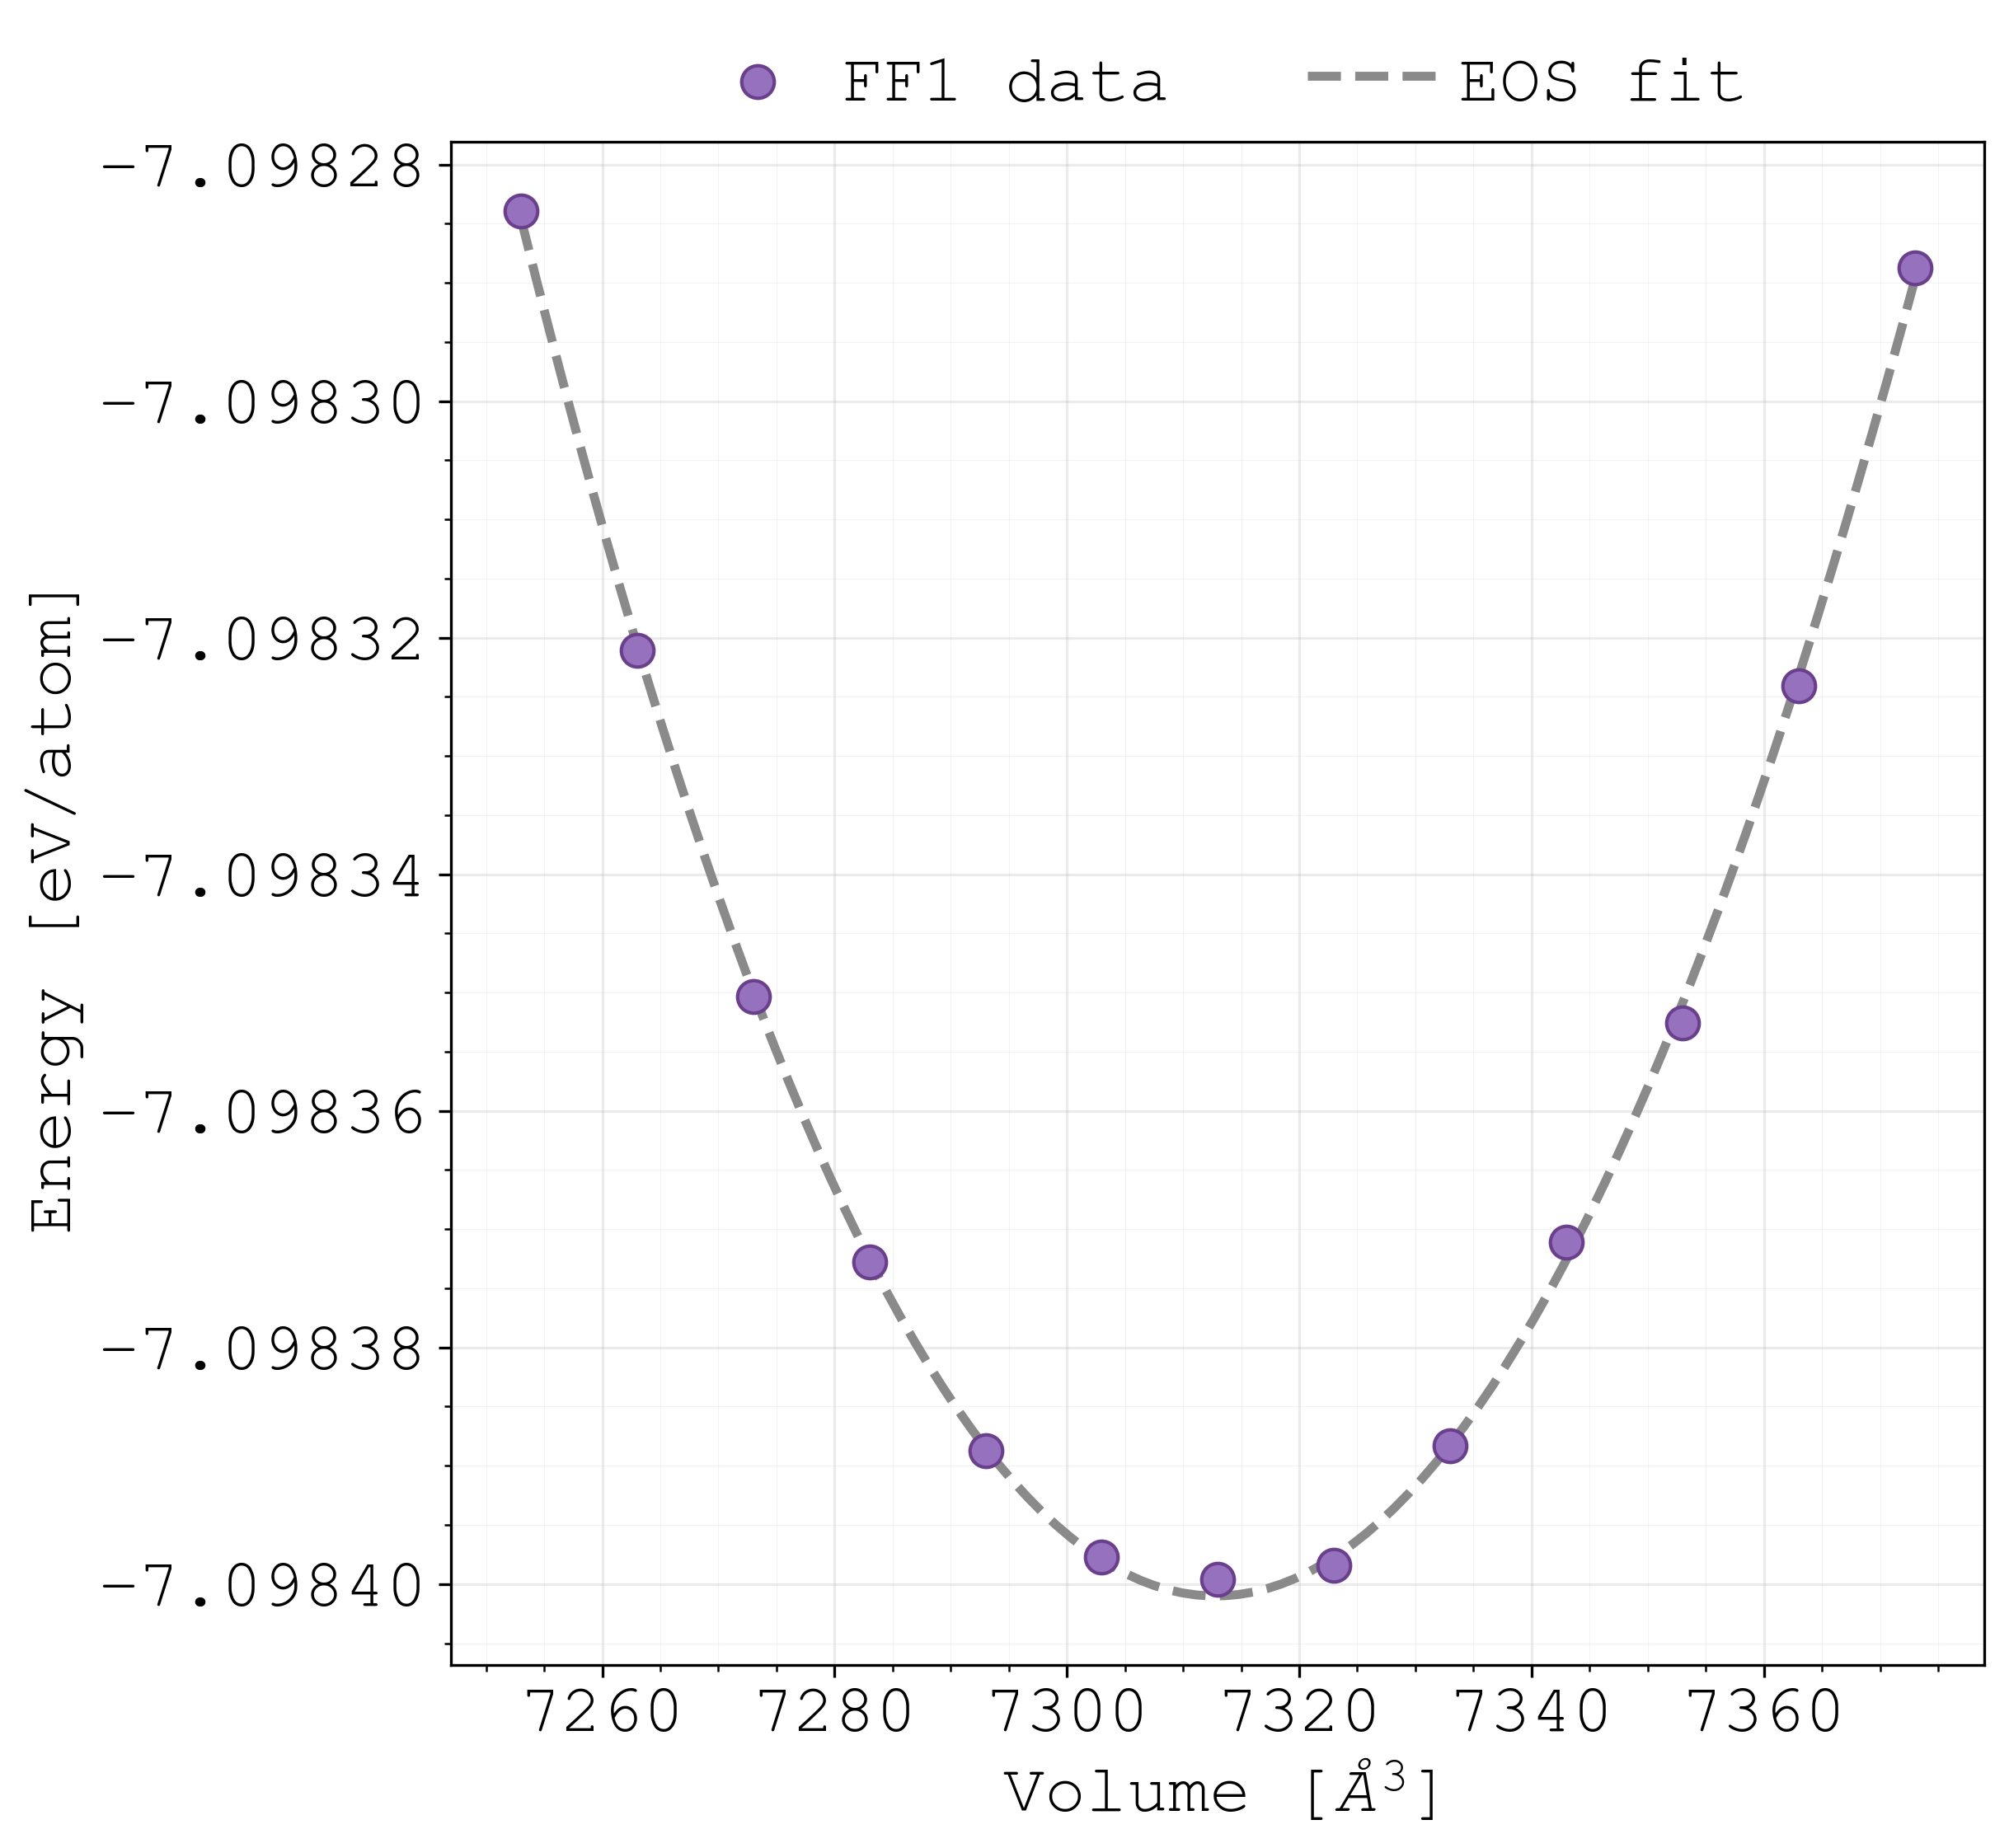
\includegraphics[width=0.7\textwidth]{EOS-FF1.png}
    \caption{
    Birch-Murnaghan equation of state (EOS) obtained by fitting the energy-volume obtained with \textbf{FF1} (red dots) for CSH. Optimal volume $V_0=7312.8$ \AA$^3$ and bulk modulus $B_0=51.14$ GPa are reported.
    }
    \label{fig:eos-ff1}
\end{figure}
\begin{figure}[H]
    \centering
    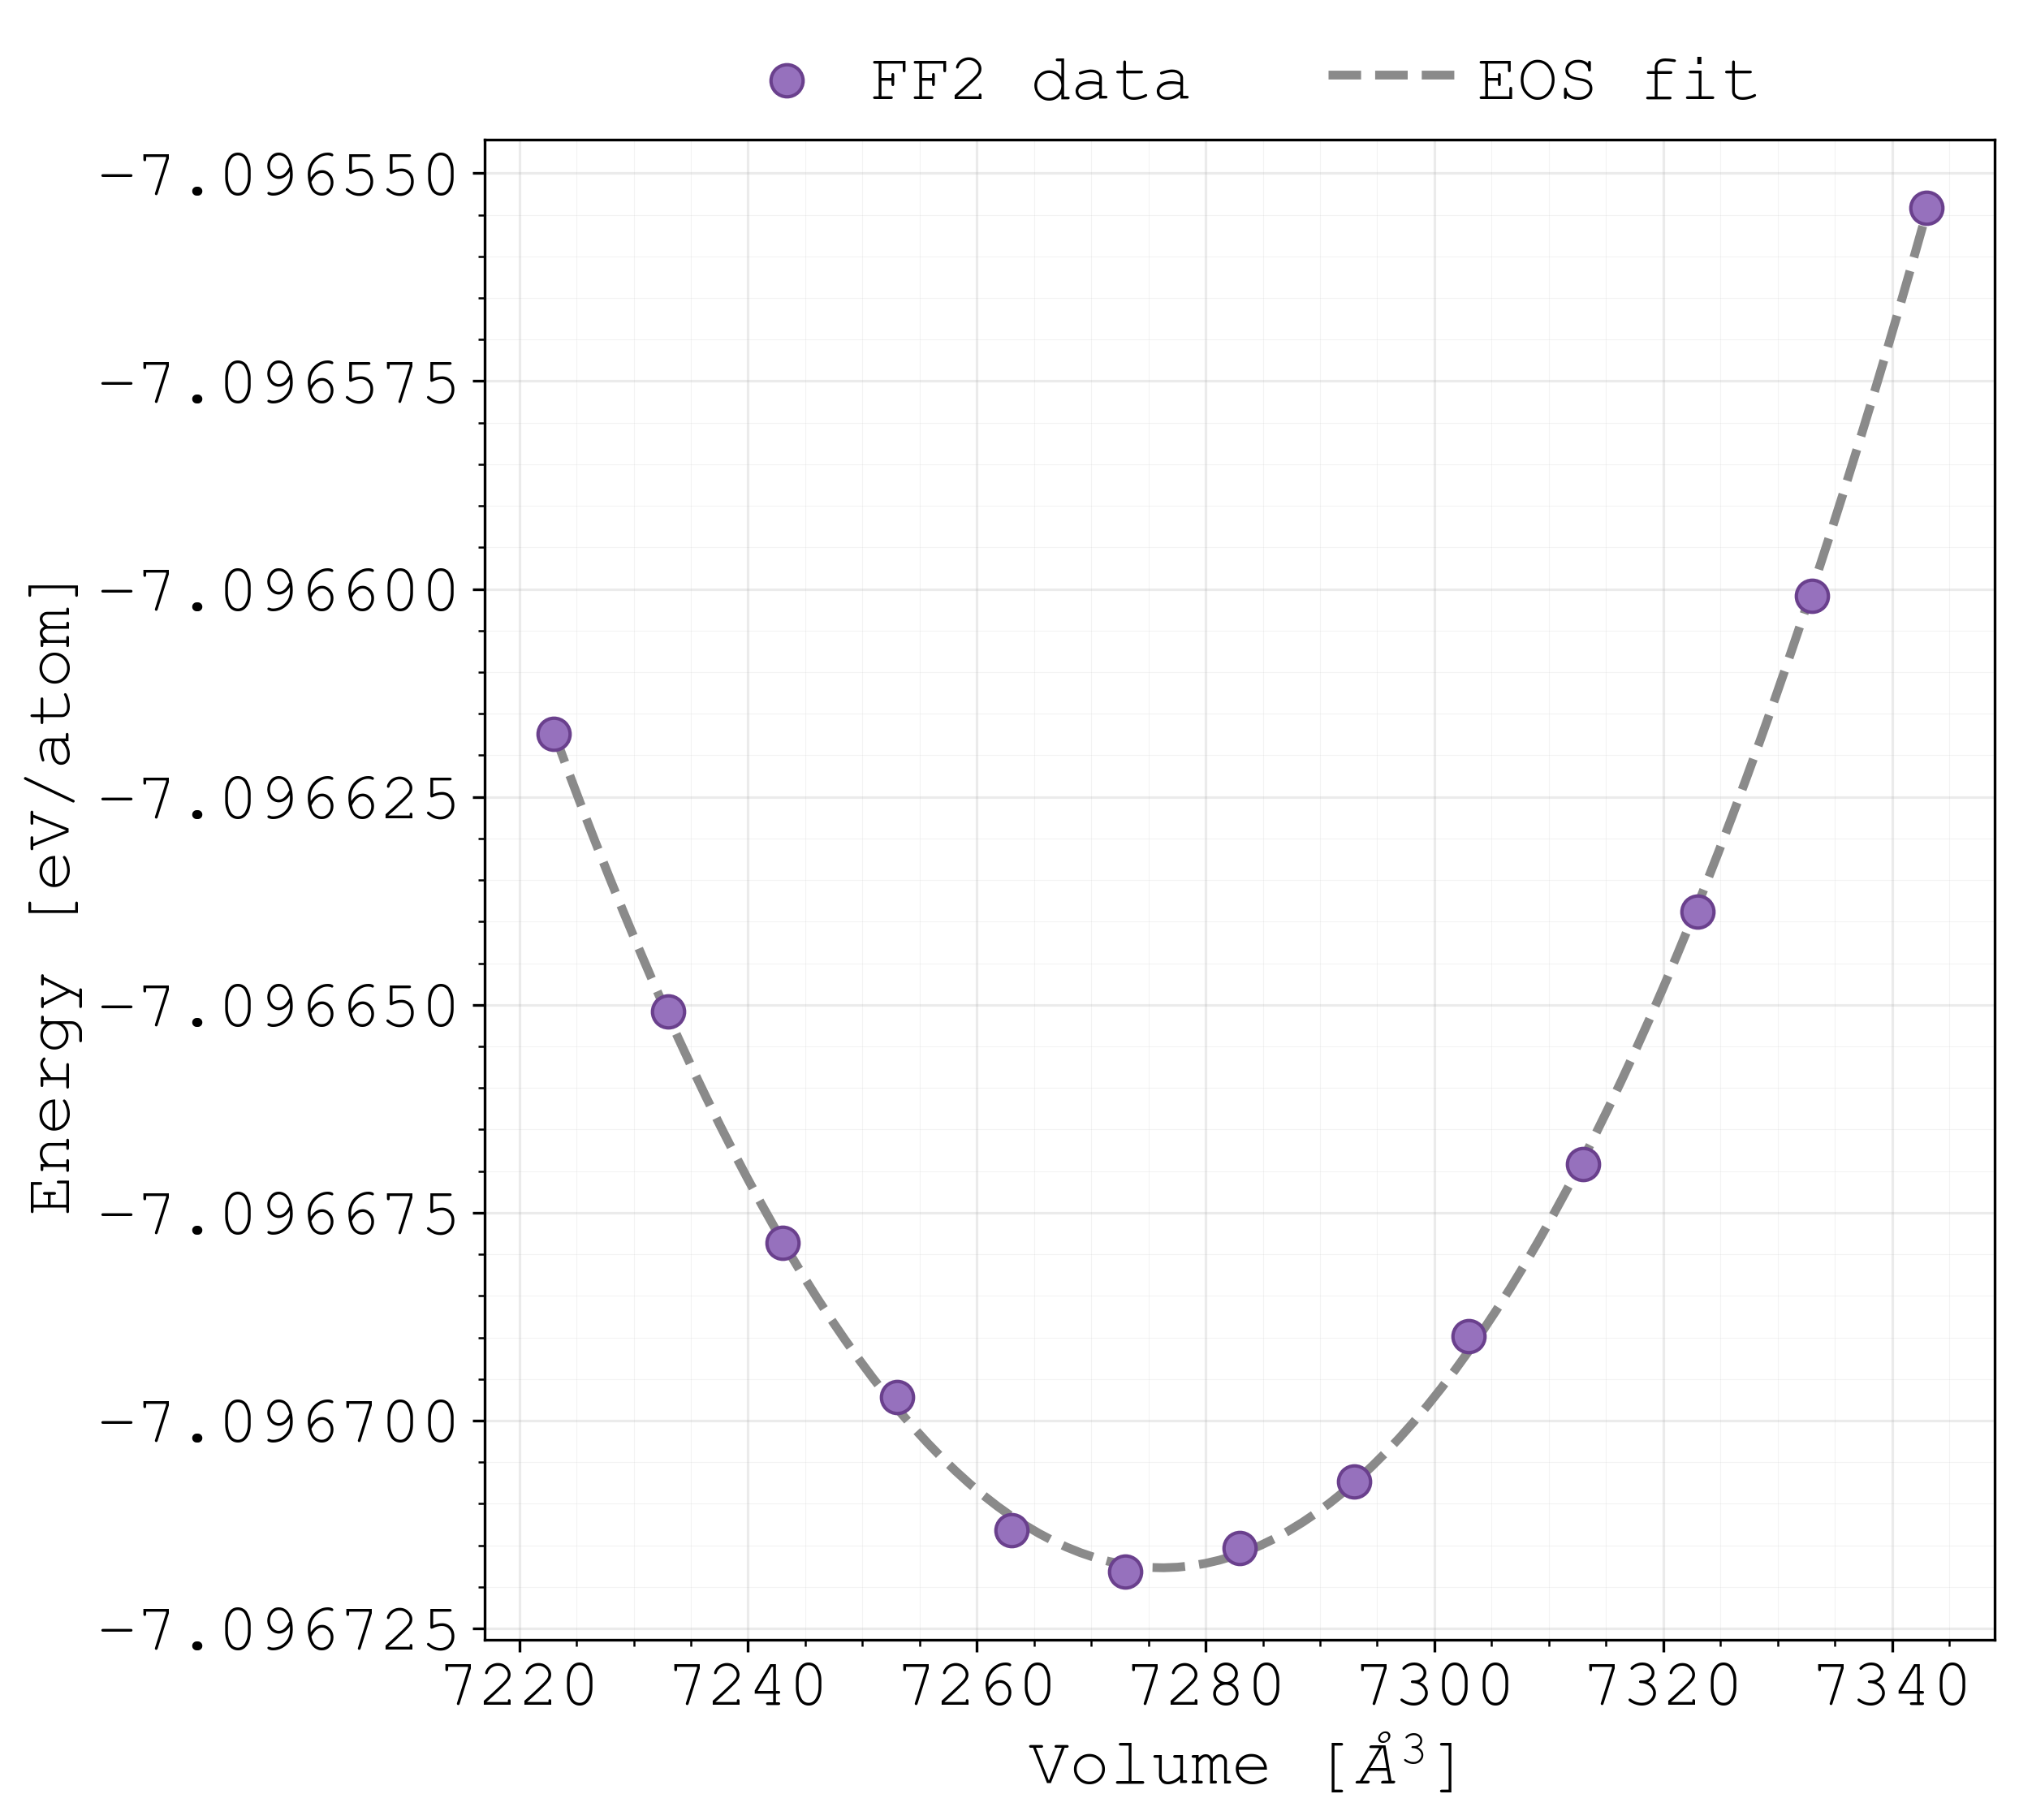
\includegraphics[width=0.7\textwidth]{EOS-FF2.png}
    \caption{
    Birch-Murnaghan equation of state (EOS) obtained by fitting the energy-volume obtained with \textbf{FF2} (red dots) for CSH. Optimal volume $V_0=7276.16$ \AA$^3$ and bulk modulus $B_0=57.88$ GPa are reported.}
    \label{fig:eos-ff2}
\end{figure}

\subsection{Simulated Annealing (SA) and EOS}
A simulated annealing (SA) procedure was applied to further optimise the CSH structure and potentially improve the bulk parameters obtained previously. During this process, the system is gradually cooled down, and as it does so, it reaches a low-energy stable configuration. Starting from the last configuration generated during the evaluation phase---which was already thermalised and stable---the SA was performed using the \textbf{FF0} force field, lowering the temperature from 400~K down to 0 K. This approach allows the system to explote a broader range of configurations, potentially leading to a more favorable state that improves the optimal bulk parameters.

Thereafter, the optimised structure was used to obtain the energy-volume data and compute the EOS, which is shown in Figure \ref{fig:eos-sa-ff0}. The optimal parameters are reported in Table \ref{tab:bulk-params}. We observe a significant increase in the optimal volume, whereas $E_0$ and $B_0$ are close to the values obtained with \textbf{FF0} and \textbf{FF1}. Finally, $B_0'$ is comparable to the value obtained with \textbf{FF1}, albeit deviating considerably from the experimental value.
\begin{figure}[H]
    \centering
    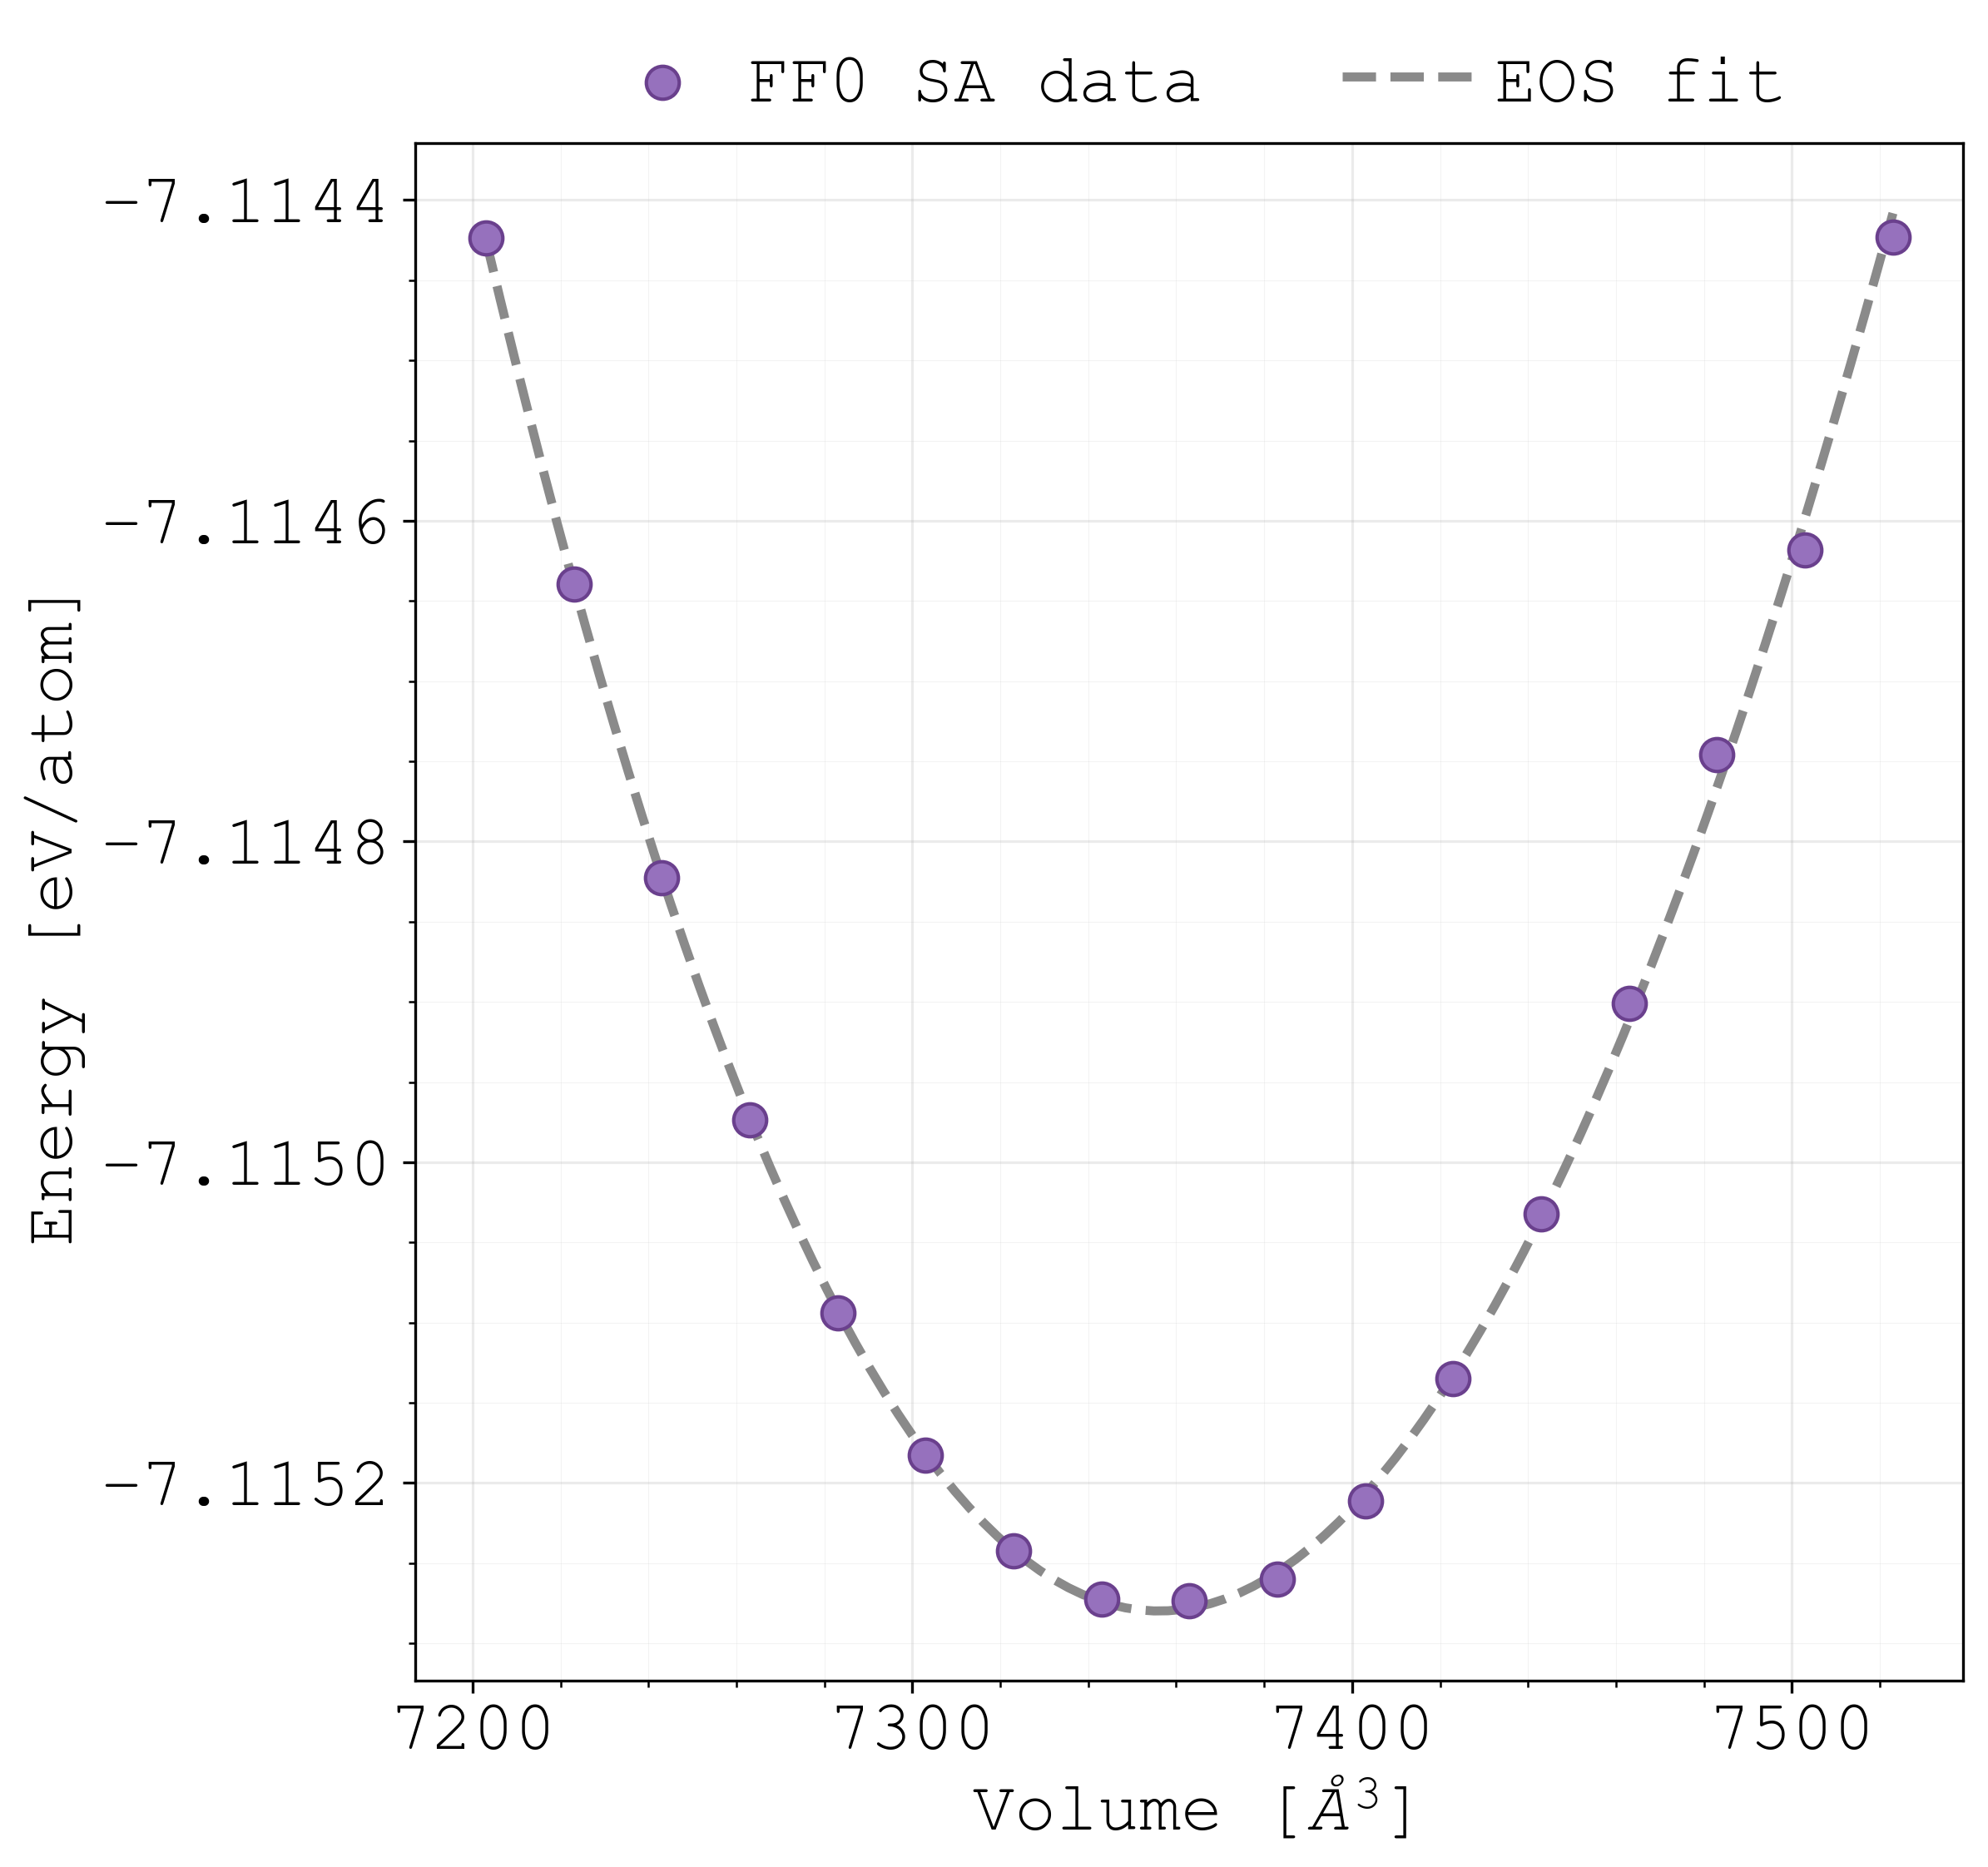
\includegraphics[width=0.7\textwidth]{EOS-SA-FF0.png}
    \caption{
    Birch-Murnaghan equation of state (EOS) obtained by fitting the energy-volume obtained with \textbf{FF0} (red dots) for CSH after the simulated annealing (SA) procedure. Optimal volume $V_0=7356.09$ \AA$^3$ and bulk modulus $B_0=55.12$ GPa are reported.
    }
    \label{fig:eos-sa-ff0}
\end{figure}

\begin{table}[h]
\centering
\caption{
    Optimal energy $E_0$, volume $V_0$, bulk modulus $B_0$ and bulk modulus derivative $B_0'$ are reported for the three MLFFs and the simulated annealing (SA) procedure. Experimental values from the literature are also included for comparison.}
\label{tab:bulk-params}
\begin{tabular}{lcccc}
\toprule
\midrule
\textbf{Model} & $V_0$ (\AA$^3$) & $E_0$ (eV) & $B_0$ (GPa) & $B_0'$ \\
\midrule
FF0       & 7302.5   & -4893.3  & 55.72      & 3.96   \\
FF1       & 7312.8   & -4897.9  & 51.14      & 9.80   \\
FF2       & 7276.2   & -4896.7  & 57.88      & -5.45  \\
FF0 SA    & 7356.1   & -4909.5  & 55.12      & 9.61   \\
Literature & N/A     & N/A      & 47 $\pm$ 3 & 4.00      \\
\midrule
\bottomrule
\end{tabular}
\end{table}



\section{Transferability of MLFFs and Thermal Expansion Coefficient of CSH}
\label{sec:transferability}
The transferability of a machine learning force field is critical to its practical utility, as it determines the model's ability to accurately predict material properties under conditions not explicitly included in the training data. In this work, we assess the transferability of \textbf{FF0} by applying it to MD simulations across a range of temperatures (200 K to 400 K) and evaluating the thermal expansion behaviour. To this end, initial structure was thermalised at each temperature for 10 ps, followed by a 20 ps MD simulation at constant temperature. The average cell volume was computed for each temperature, and then a linear fit\supercite{Xu2007} was applied to the data (see Figure \ref{expansion-coef}) yiedling the following expression:

\begin{equation}
    \label{eq:thermal-expansion}
    V(T) = 0.4724\,T + 7267.785, \quad (R^2 = 0.9435)
\end{equation}
Afterwards, the thermal expansion coefficient $\alpha_v=(1/V_0)(\partial V/\partial T)$ was computed---where $V_0$ 
was set to be the average cell volume at 200 K---yielding a value of $\alpha_v = 6.4 \times 10^{-5}$ K$^{-1}$, whereas a value of $4.5(\pm 0.9) \times 10^{-5}$ K$^{-1}$ was reported by Qomi \emph{et al.}\supercite{AbdolhosseiniQomi2015} in a numerical study of a 11-\AA tobermorite CSH model. 
Ultimately, the transferability of \textbf{FF0} is confirmed, although the thermal expansion coefficient is slightly higher than the value reported in the literature. This discrepancy likely arises from differences in model chemistry/structure, as well as the specific conditions under which such calculations were carried out. Overall, these results demonstrate the potential of MLFFs to accurately describe the underlying physics of complex systems as is the case of CSH, speeding up the calculations and enabling the exploration of larger systems and longer time scales.
\begin{figure}[H]
    \centering
    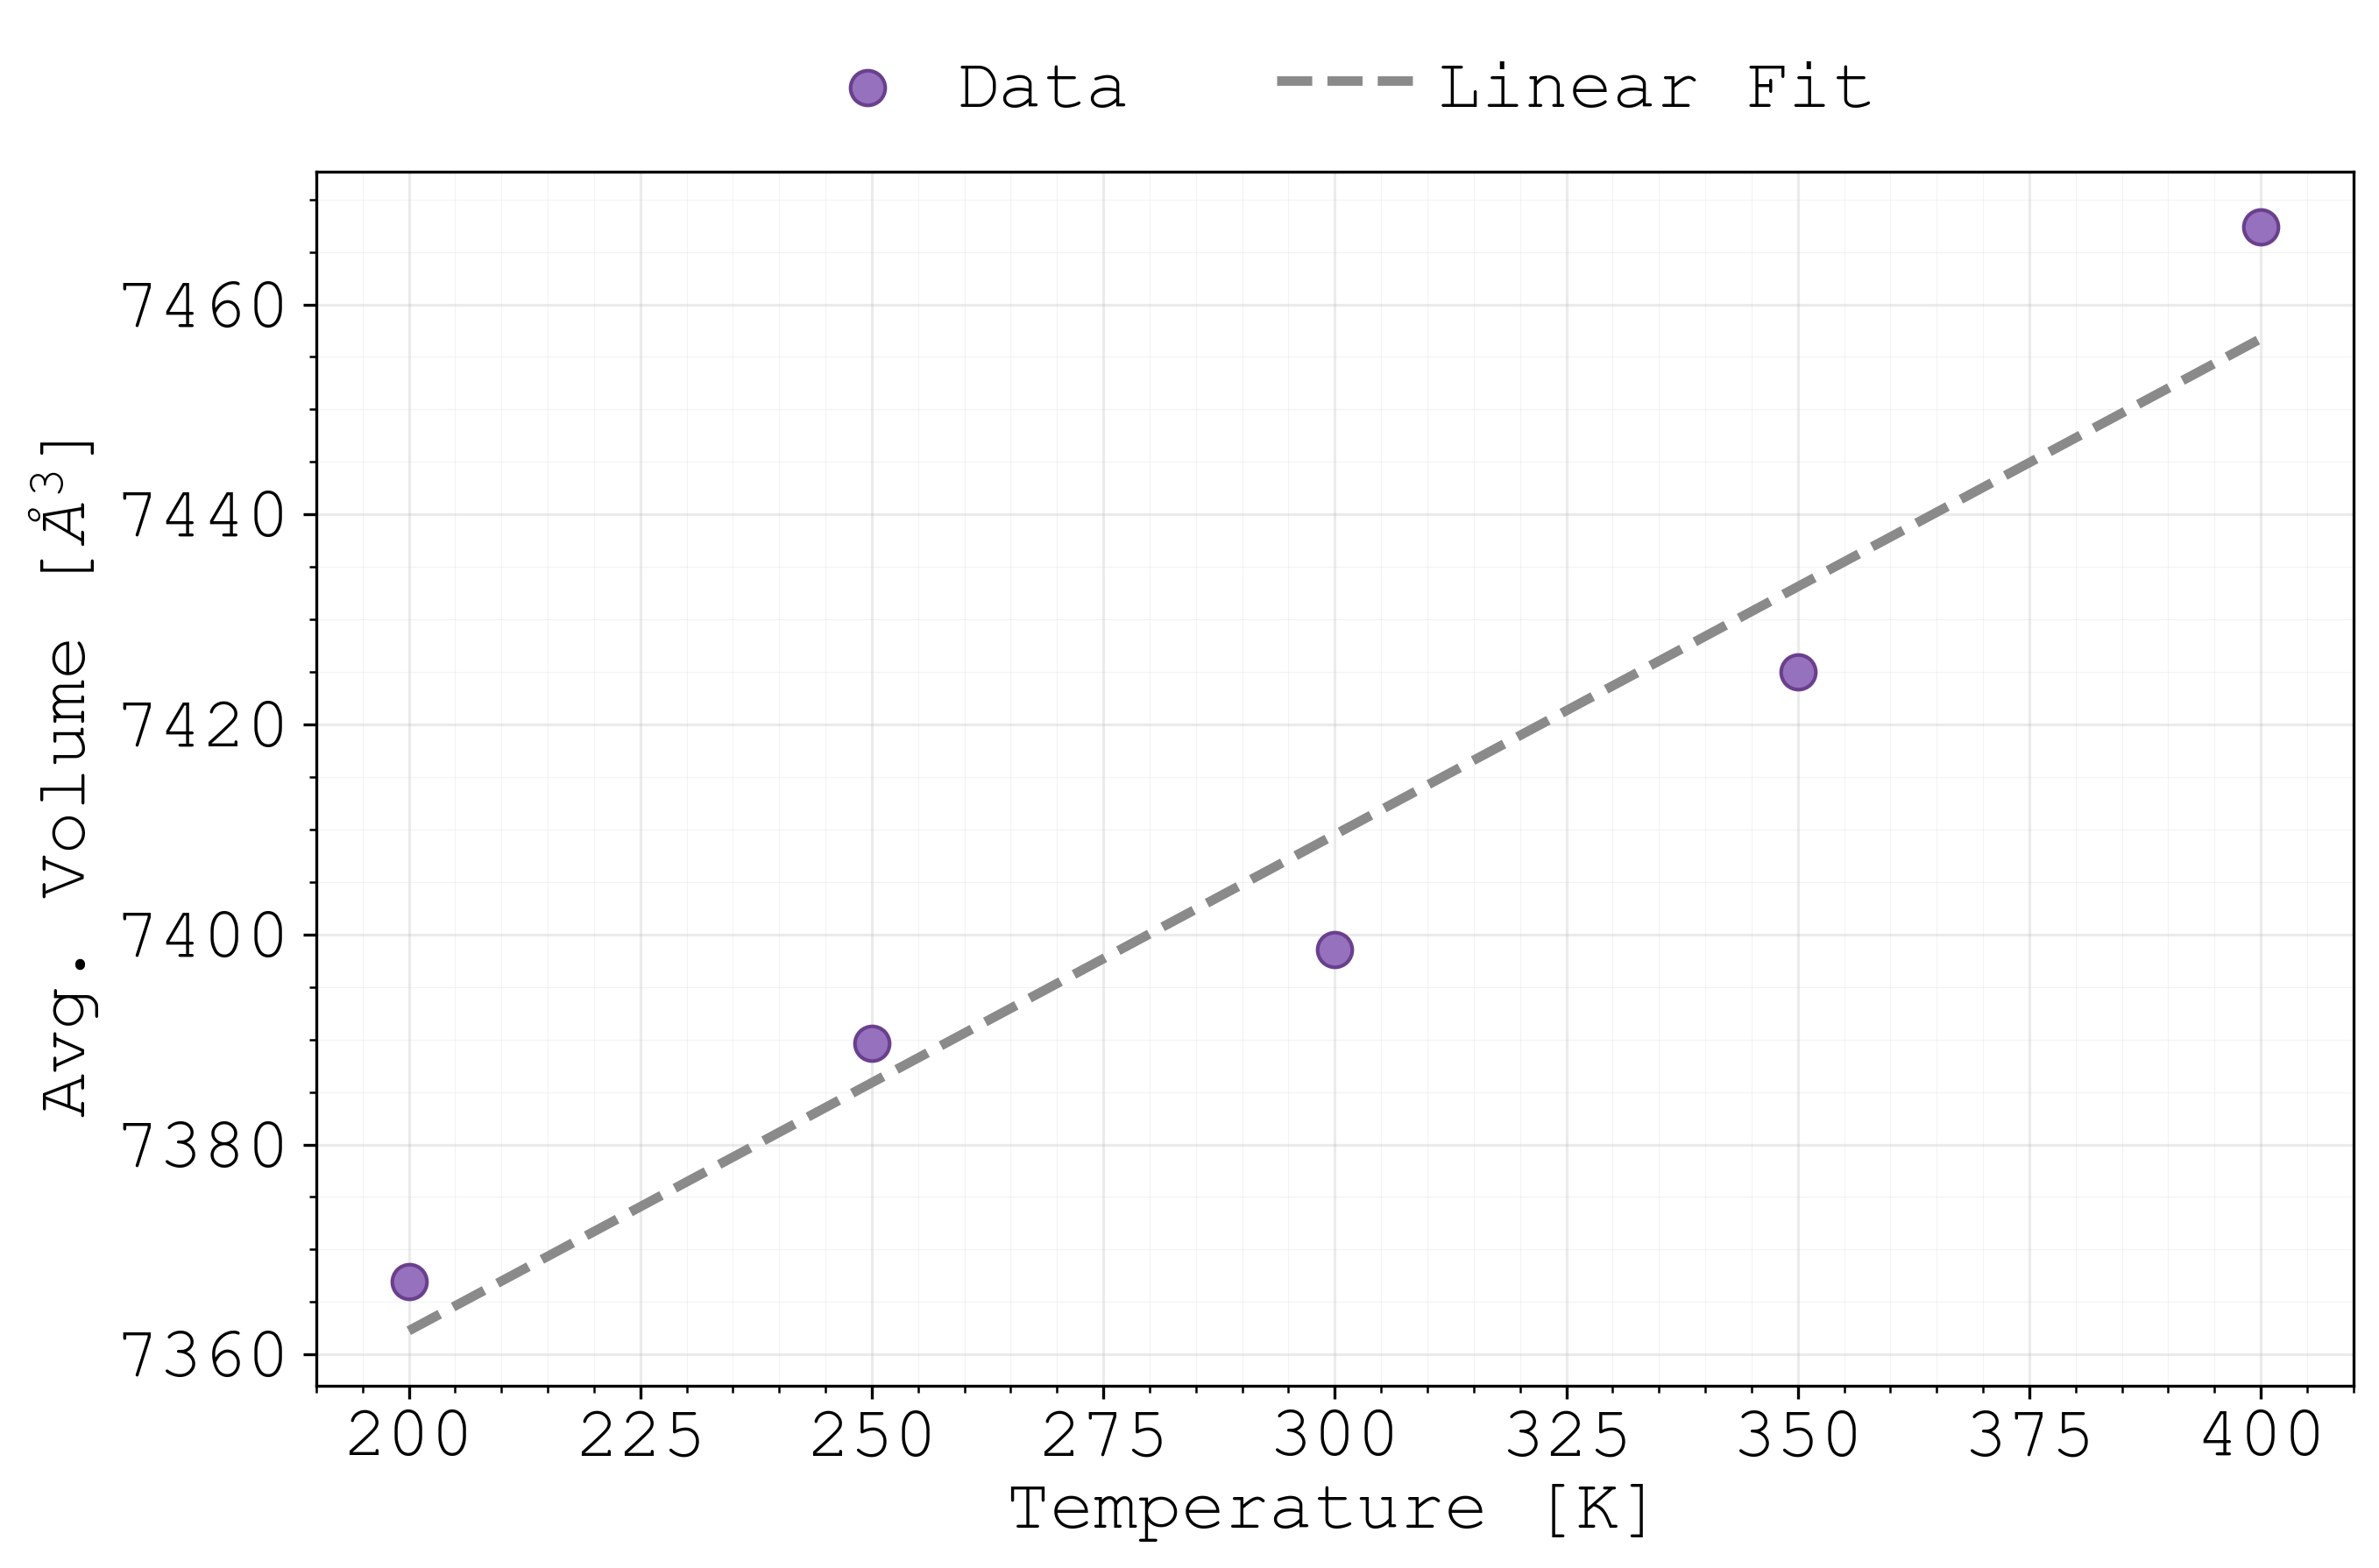
\includegraphics[width=0.8\textwidth]{expansion-coef.png}
    \caption{
    Average cell volume (purple dots) computed from MD simulations using \textbf{FF0} at 200, 250, 300, 350 and 400 K ran for 10000 steps (20 ps) each. A linear fit (dashed line) is applied to the data, 
    }
    \label{expansion-coef}
\end{figure}





